    %   Il progetto nasce dal template per il frontespizio realizzato da Marco Antonio Corallo, che ringrazio. Seguono alcuni commenti per evidenziare la presenza di alcuni pacchetti che mi sono stati utili per la stesura della tesi. Chiaramente, dipende tutto dal tipo di lavoro che uno vuole eseguire, che determina anche le diverse esigenze. Durante la stesura ho passato molto tempo su siti e forum a cercare di risolvere alcuni probelmi di formattazione, ma in generale Latex è stato piuttosto versatile. 

% Tipo di documento. L'uso di twoside implica che i capitoli inizino sempre con la prima pagina a sinistra, eventualmente lasciando una pagina vuota nel capitolo precedente. Se questa cosa è fastidiosa, è possibile rimuoverlo. 
\documentclass[a4paper, twoside,openright]{report}

% Dimensione dei margini
\usepackage[a4paper,top=3cm,bottom=3cm,left=3cm,right=3cm]{geometry} 
% Dimensione del font
\usepackage[fontsize=13pt]{scrextend}
% Lingua del testo
\usepackage[italian]{babel}
% Lingua per la bibliografia
\usepackage[fixlanguage]{babelbib}

% Codifica del testo
\usepackage[utf8]{inputenc} 
% Encoding del testo
\usepackage[T1]{fontenc}
\usepackage{lmodern}
% Permette di generare testo fittizio. Mi è stato utile 
% per capire quale sarebbe stata l'impostazione del 
% testo nella pagina prima che scrivessi un determinato paragrafo
\usepackage[dvipsnames]{xcolor}
\usepackage{lipsum}
\usepackage{tikz}
\usepackage{tikz-er2}

% Per ruotare le immagini
\usepackage{rotating}
% Per modificare l'header delle pagine 
\usepackage{fancyhdr}                     

% Uso delle immagini
\usepackage{graphicx}    
% Uso dei listing per il codice
\usepackage{listings}          
% Per inserire gli hyperlinks tra i vari elementi del testo 
\usepackage{hyperref}     
% Diversi tipi di sottolineature
\usepackage[normalem]{ulem}
\usepackage{float}
\usepackage{caption}
\usepackage[nameinlink]{cleveref}

% -----------------------------------------------------------------

% Modifica lo stile dell'header
\pagestyle{fancy}
\fancyhf{}
\lhead{\rightmark}
\rhead{\textbf{\thepage}}
\fancyfoot{}
\setlength{\headheight}{12.5pt}

% Rimuove il numero di pagina all'inizio dei capitoli
\fancypagestyle{plain}{
  \fancyfoot{}
  \fancyhead{}
  \renewcommand{\headrulewidth}{0pt}
}

% Stile del codice
\lstdefinestyle{codeStyle}{
    % Colore dei commenti
    commentstyle=\color{teal},
    % Colore delle keyword
    keywordstyle=\color{Magenta},
    % Stile dei numeri di riga
    numberstyle=\tiny\color{gray},
    % Colore delle stringhe
    stringstyle=\color{violet},
    % Dimensione e stile del testo
    basicstyle=\ttfamily\footnotesize,
    % newline solo ai whitespaces
    breakatwhitespace=false,     
    % newline si/no
    breaklines=true,                 
    % Posizione della caption, top/bottom 
    captionpos=b,                    
    % Mantiene gli spazi nel codice, utile per l'indentazione
    keepspaces=true,                 
    % Dove visualizzare i numeri di linea
    numbers=left,                    
    % Distanza tra i numeri di linea
    numbersep=5pt,                  
    % Mostra gli spazi bianchi o meno
    showspaces=false,                
    % Mostra gli spazi bianchi nelle stringhe
    showstringspaces=false,
    % Mostra i tab
    showtabs=false,
    % Dimensione dei tab
    tabsize=2,
    texcl=true
} \lstset{style=codeStyle}

% Stile di codice per dimensioni maggiori, in cui ho avuto bisogno di un testo più picolo (ad esempio se si vuole inserire del codice che ha linee molto lunghe). Per usare questo stile piuttosto che il precedente, usare 

% \lstset{style=longBlock}
%   inserire il codice...
% \lstset{style=codeStyle}

% Il secondo comando consente di tornare allo stile precedente 
\lstdefinestyle{longBlock}{
    commentstyle=\color{teal},
    keywordstyle=\color{Magenta},
    numberstyle=\tiny\color{gray},
    stringstyle=\color{violet},
    basicstyle=\ttfamily\scriptsize,
    breakatwhitespace=false,         
    breaklines=true,                 
    captionpos=b,                    
    keepspaces=true,                 
    numbers=left,                    
    numbersep=5pt,                  
    showspaces=false,                
    showstringspaces=false,
    showtabs=false,                  
    tabsize=2,
} \lstset{style=codeStyle}

\lstset{identifierstyle=\idstyle}

\makeatletter
\newcommand*\idstyle{%
	\expandafter\id@style\the\lst@token\relax
}
\def\id@style#1#2\relax{%
	\ifcat#1\relax\else
	\ifnum`#1=\uccode`#1%
	\color{blue}\bfseries
	\fi
	\fi
}

\makeatother

% Togliendo il commento al comando che segue, si inseriscono nella bibliografia anche le fonti presenti in Bibliography.bib ma non citati direttamente con il comando \cite
% \nocite{*}

% Margini prima e dopo blocchi di codice, per avere più distanza
\lstset{aboveskip=20pt,belowskip=20pt}

% Modifica dello stile dei riferimenti, con il testo in cyano
% \hypersetup{
%     colorlinks,
%     linkcolor=CornflowerBlue,
%     citecolor=CornflowerBlue
% }

% Aggiunti definizioni, teoremi, linea e listing
\newtheorem{definition}{Definizione}[section]
\newtheorem{theorem}{Teorema}[section]
\providecommand*\definitionautorefname{Definizione}
\providecommand*\theoremautorefname{Teorema}
\providecommand*{\listingautorefname}{Listing}
\providecommand*\lstnumberautorefname{Linea}

\raggedbottom

%\newcommand{\cgs}[1]{{\textcolor{brown}[\textcolor{red}{\bf{GS: }}{ \textcolor{brown}{#1]}}}}             
%\newcommand{\cmc}[1]{{\textcolor{blue}[\textcolor{magenta}{\bf{MC: }}{ \textcolor{blue}{#1]}}}}

\renewcommand{\lstlistingname}{Codice}

\crefname{section}{Sezione}{Sezioni}
\crefname{subsection}{Sezione}{Sezioni}
\crefname{chapter}{Capitolo}{Capitoli}
\crefname{figure}{Figura}{Figure}
% -----------------------------------------------------------------
\begin{document}
\definecolor{eclipseStrings}{RGB}{42,0.0,255}
\definecolor{eclipseKeywords}{RGB}{127,0,85}
\colorlet{numb}{magenta!60!black}

\lstdefinelanguage{json}{
	basicstyle=\ttfamily\footnotesize,
	commentstyle=\color{eclipseStrings}, % style of comment
	stringstyle=\color{eclipseKeywords}, % style of strings
	numbers=left,
	numberstyle=\scriptsize,
	stepnumber=1,
	numbersep=8pt,
	showstringspaces=false,
	breaklines=true,
	numberstyle=\tiny\color{gray},
	frame=lines,
	string=[s]{"}{"},
	comment=[l]{:\ "},
	morecomment=[l]{:"},
}
\begin{titlepage}
\begin{figure}[!htb]
    \centering
    
\includegraphics[keepaspectratio=true,scale=0.5]{Assets/Frontespizio/cherubinFrontespizio.eps}
\end{figure}

\begin{center}
    \LARGE{UNIVERSITÀ DI PISA}
    \vspace{5mm}
    \\ \large{DIPARTIMENTO DI INFORMATICA}
    \vspace{5mm}
    \\ \LARGE{Corso di Laurea Triennale in Informatica}
\end{center}

\vspace{15mm}
\begin{center}
    {\Large{\bf \vspace{5mm} Sviluppo di un software Flutter per acquisti online con integrazione del Backend }}
    % Se il titolo è abbastanza corto da stare su una riga, si può usare
    
    % {\LARGE{\bf Un fantastico titolo per la mia tesi!}}
\end{center}
\vspace{30mm}

\begin{minipage}[t]{0.47\textwidth}
	{\large{Relatore:}{\normalsize\vspace{3mm}
	\bf\\ \large{Prof. Claudio Gallicchio} \normalsize\vspace{3mm}}}
\end{minipage}
\hfill
\begin{minipage}[t]{0.47\textwidth}\raggedleft
	{\large{Candidato:}{\normalsize\vspace{3mm} \bf\\ \large{Gabriele Benedetti}\vspace{10mm}}}
\end{minipage}

\begin{minipage}[t]{0.47\textwidth}
	{\large{Tutor aziendale:}{\normalsize\vspace{3mm}
	\bf\\ \large{Marco Spicciani} \normalsize\vspace{3mm}}}
\end{minipage}

\vspace{20mm}
\hrulefill
\\\centering{\large{ANNO ACCADEMICO 2022/2023}}

\end{titlepage}

\tableofcontents

% Rimuovere se non si vuole la tabella delle figure
% \listoffigures

\chapter{Introduzione}
Il presente elaborato descrive il tirocinio svolto presso l'azienda 01 Informatica\cite{01info} a Pescia durante i mesi di Luglio e Agosto. L'azienda è nota per il suo impegno nel settore dello sviluppo e del mantenimento software di alta qualità, destinato a una clientela prettamente aziendale. Durante il periodo di tirocinio, mi è stato offerto di partecipare al progetto di sviluppo, design e realizzazione di un'applicazione mobile (denominata Companion) simile a una piattaforma di e-commerce, destinata a sistemi operativi Android e iOS.\\
L'obiettivo principale del progetto è stato quello di fornire agli utenti un'esperienza di "shopping virtuale" agevole e personalizzata, consentendo loro, previa esecuzione del login o accesso tramite deeplink, di acquistare una vasta gamma di prodotti, i quali possono essere aggiunti ad un carrello e, successivamente, inoltrati per l'acquisto.\\
Durante lo sviluppo di questa applicazione, è stato necessario focalizzarsi su due fondamentali componenti: il Server e il Client. Entrambi questi aspetti sono stati oggetto di un'attenta progettazione e implementazione, con l'intero processo sviluppativo affidato al sottoscritto come tirocinante presso l'azienda in questione. La sfida principale è stata quella di creare un sistema perfettamente integrato, in grado di gestire una vasta quantità di dati e transazioni, garantendo al contempo sicurezza, affidabilità e prestazioni ottimali.\\
Nel corso dell'elaborato verranno presentati i dettagli dell'architettura dell'applicazione, i metodi e le tecnologie utilizzate (sia lato Server che lato Client), si descriveranno le sfide incontrate e le scelte progettuali effettuate, illustrando i risultati ottenuti e analizzando i possibili miglioramenti futuri.

\section{Motivazioni sullo sviluppo dell'app}
La scelta di concentrarsi sull'implementazione di un'applicazione mobile è stata motivata dalla crescente diffusione e importanza degli smartphone nel panorama tecnologico contemporaneo. Tali dispositivi, infatti, hanno radicalmente trasformato le abitudini di consumo, aprendo nuove prospettive nel settore dell'e-commerce e spingendo le aziende a investire sempre di più nello sviluppo di soluzioni innovative per il mercato mobile.\\
Nello specifico, lo sviluppo di questa applicazione ha trovato le sue radici nell'esigenza di risolvere una sfida importante per le aziende, desiderose di fornire ai propri clienti un'esperienza di acquisto agevole e altamente efficiente all'interno di un catalogo prodotti pre-selezionato. Pertanto, l'applicazione è stata concepita come un "compagno" (da cui deriva appunto il suo nome "Companion") in grado di affiancare, assistere e integrare sia l'ampia gamma di prodotti già presenti sia gli utenti registrati nei Database dell'azienda. Un aspetto peculiare e innovativo, che sarà oggetto di ulteriore approfondimento, riguarda l'implementazione dei deeplink: mediante l'uso di questi collegamenti diretti, l'azienda è in grado di inviare al proprio cliente un link personalizzato, attraverso il quale è possibile automatizzare determinate operazioni (ad esempio, l'aggiunta di un prodotto specifico al carrello), rendendo l'applicazione accessibile anche ai meno esperti.\\
La riuscita nell'utilizzo di questi deeplink ha notevolmente agevolato il processo di ricerca e acquisto, permettendo ai clienti di essere guidati in modo rapido e automatico a selezionare i prodotti di interesse, senza richiedere una conoscenza approfondita dell'applicazione stessa.

\section{Guida alla relazione}
Nel presente capitolo è stata descritta una panoramica generale del contesto di svolgimento del tirocinio e del progetto proposto dall'azienda, con particolare enfasi sulle motivazioni che hanno spinto lo sviluppo dell'applicazione. Il Capitolo 2 introdurrà le tecnologie impiegate, mentre il Capitolo 3 fornirà una descrizione approfondita del processo di sviluppo dell'applicazione. Infine nel Capitolo 4 saranno presentate le considerazioni finali riguardanti l'esperienza di tirocinio, nonché le possibili prospettive di sviluppo futuro.

\chapter{Background}\label{ch:2}
Qui vengono esaminate le tecnologie e le librerie impiegate nel corso del processo di sviluppo. L'attenzione è rivolta principalmente alla comprensione dei concetti fondamentali piuttosto che alla loro implementazione pratica quindi, questo capitolo, rappresenta una risorsa di riferimento per il lettore nel caso in cui durante la lettura del \Cref{chapter_sviluppo_app} si presentino termini o concetti non completamente chiari. Inoltre, per ogni tecnologia utilizzata, ne vengono elencate (se presenti) anche le principali caratteristiche utilizzate.

\section{Tecnologie utilizzate}

\subsection{Android Studio}
Android Studio \cite{AStudio} è un software creato da Google sulla base di Intellij \cite{intellij} per aiutare gli sviluppatori a creare app per dispositivi Android. Fornisce strumenti per scrivere, testare e distribuire queste app in modo efficiente. Include un editor di codice, emulatori per provare le app su vari dispositivi, strumenti di debugging e facilita la gestione dei componenti delle app.

\subsection{Database IBM DB2 7.1}
IBM DB2 \cite{DB2} è un Relational Database Management System (RDBMS12) prodotto, appunto, dalla IBM. La prima versione risale al 1983 ed è stato uno dei primi Database a utilizzare il linguaggio SQL. La versione presente sull’AS/400 della 01 Informatica è la stessa del sistema operativo OS/400 dunque senza gli ultimi aggiornamenti della versione Server.

\subsection{Postman}
Postman \cite{postman} è una piattaforma che consente agli sviluppatori di testare e gestire le API. Postman offre un'interfaccia utente intuitiva che permette agli sviluppatori di inviare richieste HTTP alle loro API, visualizzare le risposte e analizzarle in modo dettagliato. Inoltre permette di raggruppare varie richieste ed eseguirle tutte in blocco nel modo che lo sviluppatore preferisce (in ordine casuale, in sequenza ecc.)

\subsection{Figma}
Figma \cite{figma} è un'applicazione di design collaborativo basata su cloud utilizzata per creare interfacce utente, design grafici e prototipi interattivi (mockup\footnote{I mockup sono immagini che servono a illustrare l'aspetto previsto dell'applicazione finale. Essi consentono di anticipare l'aspetto senza la necessità di scrivere il codice effettivo, fornendo una visione chiara di ciò che verrà alla fine.}). Consente a diverse persone di lavorare insieme simultaneamente sugli stessi progetti, semplificando la collaborazione nel processo di progettazione e migliorando l'efficienza nella creazione di design.

\subsection{HTTP e chiamate REST}
L'HTTP è un protocollo di comunicazione utilizzato per il trasferimento di dati tra Client e Server. REST \cite{rest}, invece, è costruito su HTTP e consente alle applicazioni e servizi web di comunicare fra loro. REST può usare qualsiasi formato di dati, ma solitamente viene utilizzato tramite JSON \cite{json}. 

\subsection{JSON Web Token}
Un JSON Web Token (JWT) \cite{jwt} è un tipo di formato JSON per rappresentare informazioni in modo sicuro. È costituito da tre parti: l'header, il payload e la firma. Il primo contiene che tipo di token e algoritmo di firma è stato usato, il payload ha le informazioni effettive e la firma verifica l'autenticità dei dati. Le informazioni non sono nascoste di default, ma possono essere criptate se necessario.

\subsubsection{Tecnica dei 2 token} \label{subsub:twotoken}
Di solito, questi token vengono impiegati per individuare il Client che inoltra la richiesta. Pertanto, uno dei principali rischi consiste nel fatto che se un individuo malintenzionato riesce ad appropriarsi di questo token, potrebbe effettuare richieste a nome del Client "hackerato". Per affrontare questa problematica, si adotta una soluzione che sfrutta l'utilizzo di due tipi di token: uno di aggiornamento e uno di accesso. Entrambi hanno una data di scadenza, ma in genere il primo persiste più a lungo (ad esempio, un mese), mentre il secondo ha un periodo di validità più breve (come qualche minuto o un'ora). Il Client utilizza il token di accesso per effettuare le richieste e, una volta scaduto, sfrutta il token di aggiornamento per ottenere un nuovo token di accesso da impiegare nelle richieste successive. Questa strategia evita di tenere il token di aggiornamento in circolazione più del necessario (dal momento che è il token di accesso a essere utilizzato più frequentemente). Inoltre, anche se uno dei token di accesso venisse compromesso, potrebbe essere sfruttato solo per un breve periodo o addirittura risulterebbe inutile per via della breve scadenza.

\subsubsection{Sicurezza}\label{subsub:secure}
Come illustrato nella sezione precedente, i token JWT possono essere sottoposti a firma attraverso l'utilizzo di una chiave simmetrica \cite{chiave_simmetrica}. Per sapere come questi token e chiavi sono stati generati, salvati sul disco, riletti e impiegati rimando il lettore alla \Cref{section_token}. Nel contesto attuale, forniremo solo spiegazioni in merito alla classe utilizzata e agli algoritmi impiegati, definendone la natura e motivando le ragioni della loro scelta.

\paragraph{Cipher}
Cipher \cite{cipher} è una classe Java che è utilizzata per sfruttare gli algoritmi di cifratura e decifratura per proteggere i dati sensibili.
Questa classe consente di creare un oggetto di tipo Cipher che può essere configurato con un algoritmo di cifratura specifico (come AES, DES, RSA, ecc.), una modalità operativa (come CBC, ECB, CTR, ecc.) e una possibile opzione di riempimento (come PKCS5PADDING). Una volta configurata correttamente, si può utilizzare l'oggetto Cipher per cifrare i dati (testo, byte, etc.) con una chiave e decifrarli successivamente utilizzando la stessa chiave.

\paragraph{MessageDigest}
La classe MessageDigest \cite{message_digest} in Java viene utilizzata per calcolare hash \cite{hash} crittografici di dati, come ad esempio MD5 o SHA-256. La differenza principale con la classe Cipher è che MessageDigest non può decriptare i dati in quanto il suo utilizzo è strettamente legato all hashing unidirezionale dei dati.

\paragraph{HMAC e SHA-256}
HMAC \cite{hmac} è un metodo di autenticazione basato su hashing che viene utilizzato per verificare l'integrità e l'autenticità dei dati. Questo processo coinvolge una chiave segreta e una funzione hash. L'HMAC prende in input il dato, lo combina con la chiave segreta e passa tutto ad una funzione hash (ad esempio SHA-256) per generare un valore di autenticazione. Questo valore viene quindi confrontato in seguito con il valore ricevuto per determinare se i dati sono stati modificati o falsificati. Di fatto, basta una piccola modifica all'input originale che la funziona hash cambia radicalmente ("avalanche effect")

\paragraph{AES, ECB e PKCS5PADDING}
AES \cite{aes} rappresenta un algoritmo di cifratura a blocchi basato su chiave simmetrica, il quale sfrutta la medesima chiave sia per la criptazione che per la decriptazione dei dati. E' considerato tra gli standard più affidabili per la protezione dei dati in quanto offre differenti lunghezze di chiave (128, 192 o 256 bit) per adattarsi alle necessità di sicurezza.
La procedura di cifratura avviene seguendo la tecnica ECB (Electronic Codebook) \cite{ecb}, in cui l'input da cifrare viene suddiviso in blocchi che vengono successivamente crittografati individualmente, sfruttando la stessa chiave. Nel caso in cui questi blocchi non corrispondano alla dimensione prescritta dall'algoritmo AES, si fa ricorso alla tecnica di riempimento PKCS5PADDING per "riempire" i blocchi prima della cifratura.
È fondamentale notare che l'approccio ECB non è consigliato per l'uso in scenari di produzione, poiché la cifratura di blocchi identici genera lo stesso testo cifrato, potenzialmente esponendo a vulnerabilità. Tuttavia, per scopi didattici, è stato scelto di adottare l'algoritmo ECB per la sua semplicità, dato che non richiede l'utilizzo di un IV (Initialization Vector \cite{iv}).

\subsection{Flutter} \label{sub:flutter}
Flutter \cite{flutter} è un framework creato da Google per lo sviluppo di applicazioni cross-platform. Utilizza il linguaggio di programmazione Dart e consente agli sviluppatori di creare app con una singola base di codice che può essere eseguita su diverse piattaforme, come nel nostro caso iOS e Android. Flutter si concentra sull'interfaccia utente e offre un'ampia gamma di Widget \cite{widget} personalizzabili per creare app con un aspetto nativo e prestazioni elevate. Di seguito vengono spiegati i Widget utilizzati più frequentemente.

\subsubsection{Scaffold} \label{subsub:scaffold}
Lo Scaffold \cite{scaffold} è un Widget Flutter che implementa una struttura visiva base in accordo con le linee guida del Material Design. Lo Scaffold infatti permette di posizionare correttamente gli elementi all'interno della schermata in modo che non si sovrappongano con altri elementi del sistema e dà la possibilità di inserire Widget molto noti quali l'AppBar, il Drawer, la barra di navigazione in basso eccetera. Diciamo che si può vedere come il componente padre di tutto.

\subsubsection{Expanded} \label{subsub:expanded}
Expanded \cite{expanded} è un Widget che permette a tutti i figli di espandersi orizzontalmente e/o verticalmente in modo da riempire tutto lo spazio possibile. L'ampio impiego di questo widget è motivato dalla necessità che l'applicazione sia responsive e quindi in grado di adattarsi alle varie dimensioni degli schermi mobile. Con il termine "espandersi" è inteso che il Widget figlio incrementa la sua altezza o larghezza fino a che è possibile farlo.

\subsubsection{ListView}
ListView \cite{listview} è un Widget Flutter che permette di creare liste scorrevoli. Nello specifico, è stato impiegato il costruttore 'ListView.builder()', che consente di generare liste senza limiti predefiniti e che renderizza solamente gli elementi visibili in quel momento. Ciò non solo assicura efficienza nell'utilizzo delle risorse, ma riduce anche il consumo energetico complessivo dell'applicazione.

\subsubsection{Go Router} \label{subsub:go_router}
Go Router \cite{gorouter_lib} è la libreria principale utilizzata per la navigazione tra le schermate e per la ricezione dei deeplink. Attraverso questa libreria è possibile definire rotte personalizzate, corrispondenti di fatto a delle URI \cite{uri}, le quali vengono in seguito identificate dal sistema sottostante nel momento in cui l'utente desidera sfruttare una specifica URI.

\subsubsection{TextField} \label{subsub:textfield}
In Flutter, il TextField \cite{textfield} è un'area in cui gli utenti possono scrivere del testo usando la tastiera fisica o virtuale. Per gestire il testo e le interazioni, si usa il TextEditingController, che permette tra le tante cose di impostare il testo iniziale, leggere quello inserito dagli utenti, modificarlo e reagire ai cambiamenti. In poche parole, il TextField è dove il testo viene inserito e il TextEditingController è l'oggetto che rappresenta il testo dentro il TextField.

\begin{figure}[H]
	\centering
	\makebox[\textwidth] [c]{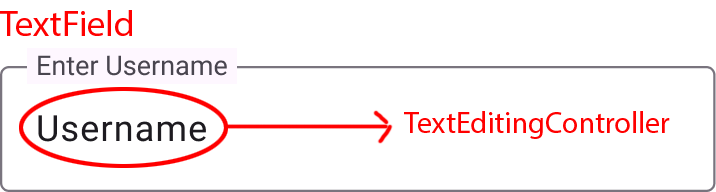
\includegraphics[width=0.5\linewidth, keepaspectratio]{Assets/Username_Field_verbose.png}}
	\caption{Rappresentazione grafica del TextField}
	\label{fig:textfield_verbose}
\end{figure}
\noindent

\subsubsection{Provider} \label{subsub:provider}
Provider \cite{provider} è una classe Flutter che gestisce la condivisione dei dati tra Widget. Questa classe permette di posizionarsi in modo globale all'interno dell'applicazione in modo che possa essere accessibile da chiunque e in qualunque punto dell'applicazione. Un aspetto importante è inoltre la sua capacità di agire come intermediario tra i Widget: quando un componente desidera apportare modifiche a qualcosa al di fuori del proprio scope, può richiedere al "Provider" di notificare direttamente l'elemento interessato affinché si "aggiorni". Per meglio comprendere questo concetto, esaminiamo il seguente esempio:
\begin{figure}[H]
	\centering
	\makebox[\textwidth] [c]{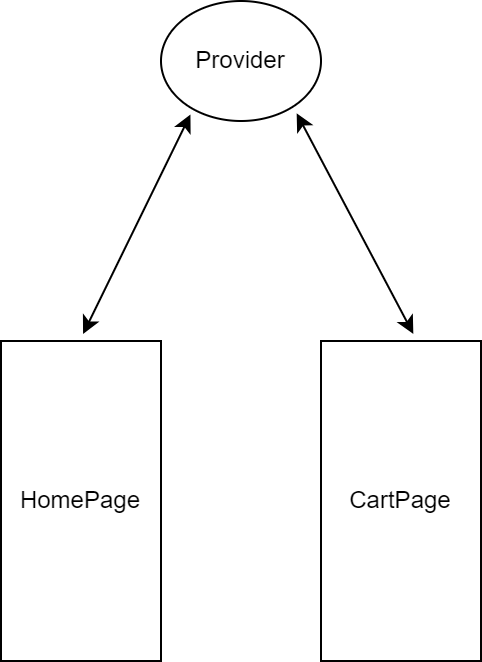
\includegraphics[width=0.5\linewidth, keepaspectratio]{Assets/diagram 1.png}}
	\caption{Rappresentazione grafica del Provider come intermediario}
	\label{fig:provider_example1}
\end{figure}
\noindent
Com'è facilmente intuibile, prendendo come esempio la pagina "Home" e del "Carrello", il Provider si comporta come intermediario tra le 2, essendo una classe a portata globale.\\
Immaginiamo ora che queste due pagine desiderino condividere una lista, specificamente l'elenco dei prodotti che l'utente ricerca e seleziona. Quando questo si trova nella pagina "Home" e aggiunge un elemento a questa lista, il "Provider" avvertirà la pagina del "Carrello" che è stato aggiunto un nuovo elemento. Di conseguenza, la pagina del "Carrello" si aggiornerà con i nuovi dati. Questa dinamica può essere illustrata nel seguente schema:
\begin{figure}[H]
	\centering
	\makebox[\textwidth] [c]{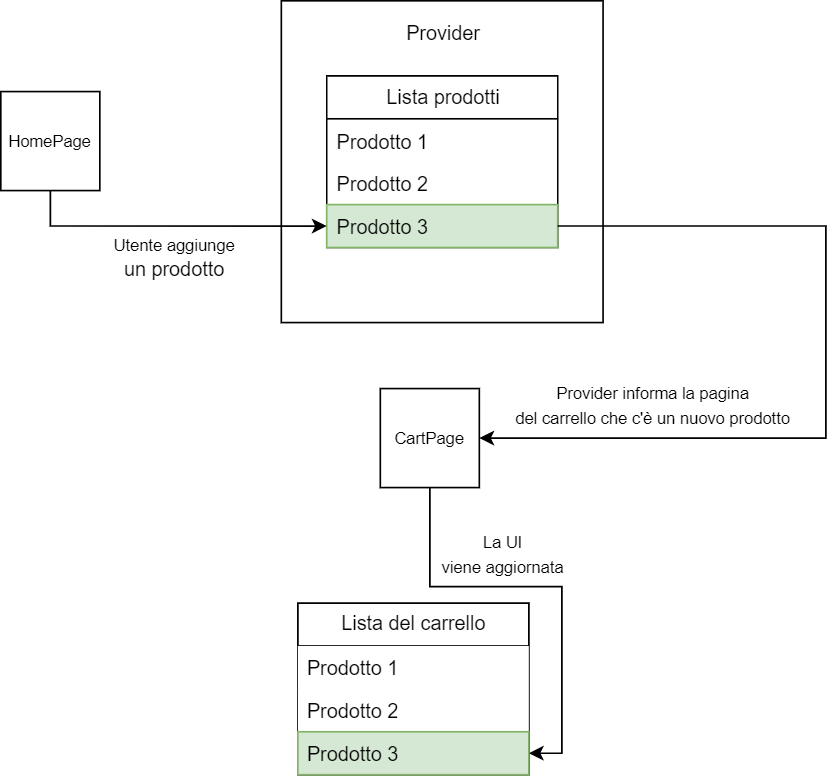
\includegraphics[width=1\linewidth, keepaspectratio]{Assets/diagram 2.png}}
	\caption{Condivisione dei dati e aggiornamento UI}
	\label{fig:provider_example2}
\end{figure}

\noindent
Tuttavia, questo Widget non è solo utile per condividere dati tra diverse pagine, ma anche tra componenti all'interno della stessa pagina. Dato che Flutter è fortemente orientato ai Widget, spesso accade che due di questi siano definiti in file separati, il che può rendere complicata la comunicazione tra componenti interni situati in Widget diversi. Prendiamo ad esempio la pagina del carrello, composta da due Widget: una lista e un testo che indica il totale dell'importo. Per farli comunicare efficacemente, essendo situati in due scope differenti, si può fare uso del "Provider". Quando l'utente modifica, ad esempio, la quantità di un prodotto, la lista imposta nel "Provider" il nuovo "importo totale" e il "Provider" si occuperà di notificare al "Widget testo" di aggiornarsi con il nuovo valore. Questa dinamica può essere chiaramente rappresentata attraverso il seguente schema:
\begin{figure}[H]
	\centering
	\makebox[\textwidth] [c]{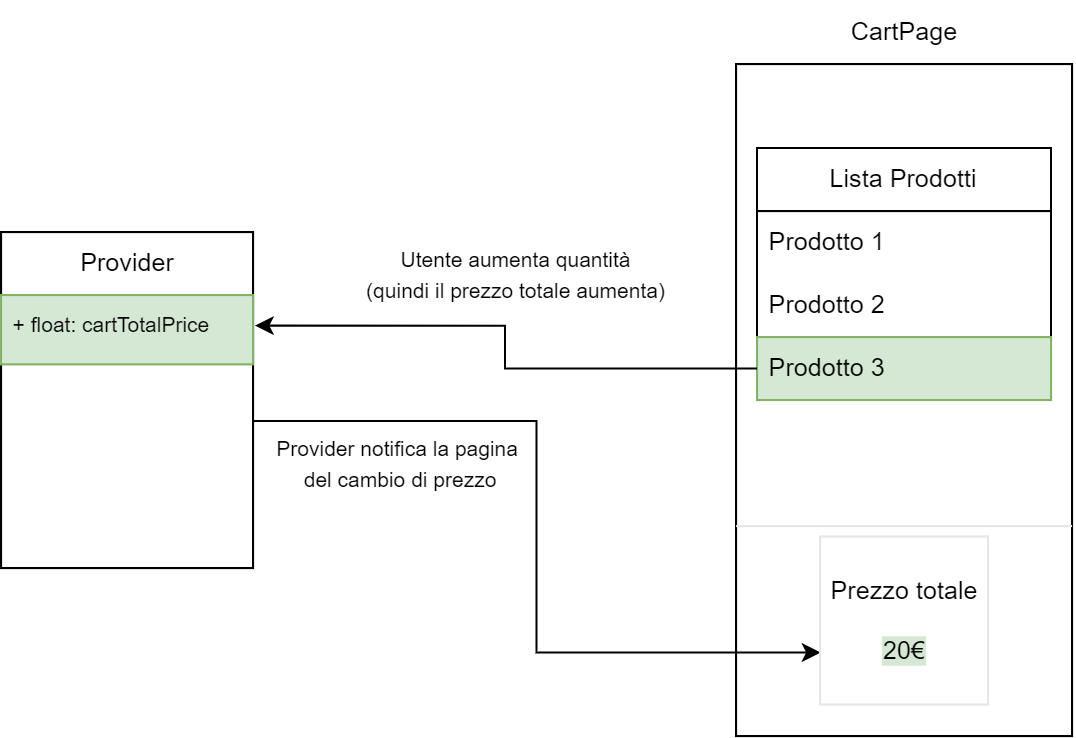
\includegraphics[width=1\linewidth, keepaspectratio]{Assets/diagram 3.png}}
	\caption{Condivisione dei dati tra componenti interni}
	\label{fig:provider_example3}
\end{figure}

\noindent

\paragraph{Selector}
Per consentire al "Provider" di individuare quale Widget deve essere aggiornato, è essenziale inserire il componente interessato dentro un "Selector" \cite{selector}. Questo Widget consente di specificare quale variabile del "Provider" deve essere monitorata. In tal modo, quando il "Provider" emette una notifica di cambiamento, il "Selector" verifica se l'aggiornamento riguarda la variabile monitorata e, in caso affermativo, aggiorna il componente con il nuovo valore.

\subsubsection{FutureBuilder} \label{subsub:futurebuilder}
Questo Widget è stato progettato per gestire le operazioni asincrone in modo semplice ed efficace, consentendo lo sviluppo di interfacce utente reattive e fluide. Il suo scopo principale è quello di semplificare l'integrazione dei dati asincroni, come il recupero di informazioni da Server o Database, all'interno dell'interfaccia utente. Il FutureBuilder \cite{future_builder} accetta un "future" come input, che rappresenta un'operazione (cioè una funzione) che potrebbe richiedere del tempo per essere completata. Durante l'attesa del completamento, il FutureBuilder è in grado di mostrare un'interfaccia temporanea, come un caricamento o una schermata con dati iniziali, in modo da non bloccare l'interfaccia durante il caricamento dei dati.

\subsubsection{FadeInImage} \label{subsub:fadeinimage}
FadeInImage \cite{fadeinimage} è un Widget Flutter la cui funzione principale è quella di sostituire gradualmente un'immagine di placeholder con un immagine finale, ottenuta da un URL. Il FadeInImage richiede due immagini come input: un'immagine di "placeholder" da visualizzare inizialmente, mentre l'immagine finale è in corso di caricamento, e quella effettiva che verrà mostrata una volta scaricata. Quando è finito lo scaricamento, il FadeInImage applicherà un effetto di dissolvenza graduale tra queste due immagini, creando un effetto visivo piacevole e delicato.

\section{Librerie impiegate}
\subsection{Javalin}
Javalin \cite{javalin} è un framework web scritto in linguaggio di programmazione Java, progettato per semplificare lo sviluppo di applicazioni web. Si concentra sulla semplicità e facilità d'uso, offrendo uno strato di astrazione per gestire le richieste HTTP e le risposte in modo pulito ed efficiente. Sebbene sia minimalista, Javalin offre ancora funzionalità essenziali come il routing delle richieste, la gestione dei parametri, il supporto per la creazione di endpoint RESTful e la gestione dei middleware.

\subsection{JWT} \label{sub:jwt}
JWT \cite{JWT_lib} è la libreria ufficiale che permette la creazione di token firmati mediante semplici metodi. Questa libreria è stata usata, per l appunto, per creare i token e verificarli una volta ricevuti dal Client.

\subsection{JUnit}
JUnit \cite{junit} è un framework di test unitari per il linguaggio di programmazione Java. Esso fornisce una struttura per scrivere, eseguire e organizzare test automatizzati per verificare il corretto funzionamento delle singole unità di codice, come metodi o classi, in isolamento dal resto dell'applicazione.
Il framework offre annotazioni, asserzioni e metodi di configurazione che semplificano il processo di scrittura e l'esecuzione dei test. Questa libreria è stata usata in quanto richiesta dal mio tutor aziendale.

\subsection{GSON}
GSON \cite{gson} è una libreria di Google che permette di convertire/serializzare un oggetto Java in testo JSON mediante dei semplici metodi ".toJson()" e ".fromJson()".

\subsection{SQLite}
SQLite \cite{sqlite} è una libreria che permette l'utilizzo di Database senza avere un vero e proprio DBMS. Di fatto, viene salvato tutto in file locali ed è possibile utilizzare il linguaggio SQL per gestire e manipolare le tabelle. Questa libreria consente quindi di avere un vero e proprio Database locale nel quale salvare i dati importanti in modo facile e veloce.

\subsection{Lottie}
Lottie \cite{lottie} è la libreria ufficiale sviluppata dall'azienda "Lottie" che permette di visualizzare le animazioni scaricate dal sito, in formato JSON, dentro ai Widget.

\paragraph{Material Dialog}
Material Dialog \cite{material_dialog} è la libreria che fa uso di Lottie per mostrare dei dialog animati comprensivi di titolo, descrizione e pulsanti a scelta.
\chapter{Sviluppo dell'applicazione} \label{chapter_sviluppo_app}
In conformità con i requisiti stabiliti, il Server si avvale di un Database dotato di tabelle pre-caricate, destinato a memorizzare informazioni riguardanti ordini, testate e utenti. Le richieste HTTP vengono gestite attraverso il framework Javalin (vedi \Cref{subsub:javalin}), il quale assicura un'elevata efficienza e affidabilità nella gestione delle interazioni tra Client e Server.\\
Dal canto suo, il Client è stato attentamente disegnato e progettato in risposta alle specifiche fornite dal tutor aziendale, il quale ha espressamente richiesto un'esperienza di navigazione sobria e incentrata sull'essenziale. In particolare è stato espresso l'importante desiderio che la pagina home dell'applicazione si presenti in modo pulito e minimale, senza suggerimenti di prodotti o elementi superflui. Pertanto, l'interfaccia principale dell'applicazione sarà caratterizzata da una pagina vuota, arricchita solamente da una barra di ricerca ben visibile, il cui scopo è facilitare l'accesso rapido e intuitivo alla vasta gamma di prodotti offerti nel catalogo. Successivamente è stata espressa la necessità di includere, sempre nella pagina home, la visualizzazione tramite lista non ordinata dei prodotti disponibili, oltre a un'altra pagina destinata a mostrare, con lista ordinata per data di aggiunta, i prodotti presenti nel carrello. Infine è stato richiesto un sistema di deeplink, capace di sfruttare il nome dell'azienda e caratterizzato da un insieme di funzionalità particolari:
\begin{itemize}
	\item \textbf{Token di Riconoscimento Utente:} Ogni deeplink \underline{deve} contenere il token JWT di riconoscimento di ogni utente inserito nel Database. Questo token sarà utilizzato per identificare in modo univoco l'utente durante la richiesta, consentendo l'accesso a servizi personalizzati e proteggendo i dati sensibili.
	\item \textbf{Login Automatico per Utenti non Autenticati:} Nel caso in cui un utente non abbia effettuato il login, ma desideri comunque accedere all'applicativo e compiere azioni specifiche, ad esempio effettuare acquisti, il sistema fornirà un meccanismo di login automatico persistente. Cliccando sul deeplink, infatti, l'utente eseguirà la richiesta di login in modo automatico ad offrire un'esperienza semplice e con soluzione di continuità.
	\item \textbf{Link per Aggiunta Automatica al Carrello:} Al fine di semplificare l'esperienza di acquisto, l'applicazione fornirà un deeplink dedicato che permetterà all'utente di aggiungere automaticamente un prodotto specifico al carrello con una determinata quantità.
\end{itemize}

\noindent
Esempio di deeplink che permette di aggiungere un determinato prodotto con id "1340" e quantità "10":
\begin{lstlisting}
	info01://codice01.companion.it/token/code=1340/quantity=10
\end{lstlisting}

\section{Server}\label{section1}
Il Server è stato implementato in Java e utilizza il framework Javalin per mettersi in ascolto su una porta predefinita, accettando e gestendo le richieste HTTP provenienti dai Client. Tutte le interrogazioni in entrata sono sottoposte a un attento processo di analisi e filtraggio, al fine di garantire l'aderenza agli standard definiti dallo sviluppatore. Di fatto, qualsiasi richiesta che non sia conforme a tali standard viene prontamente ignorata e scartata per garantire la sicurezza e l'integrità del sistema.\\
Per essere considerata valida, una richiesta deve almeno includere il token di accesso o il token di aggiornamento nell header, a meno che non si tratti specificamente di una richiesta di accesso al sistema. In quest'ultimo caso, il processo di autenticazione viene innescato e, una volta completato con successo, il Server risponde inviando al Client i token di accesso e di aggiornamento, come precedentemente stabilito nella \Cref{subsub:twotoken} del presente elaborato.

\subsection{Database: Analisi e Struttura} \label{section2}
\begin{figure}
	\centering
	\makebox[\textwidth] [c]{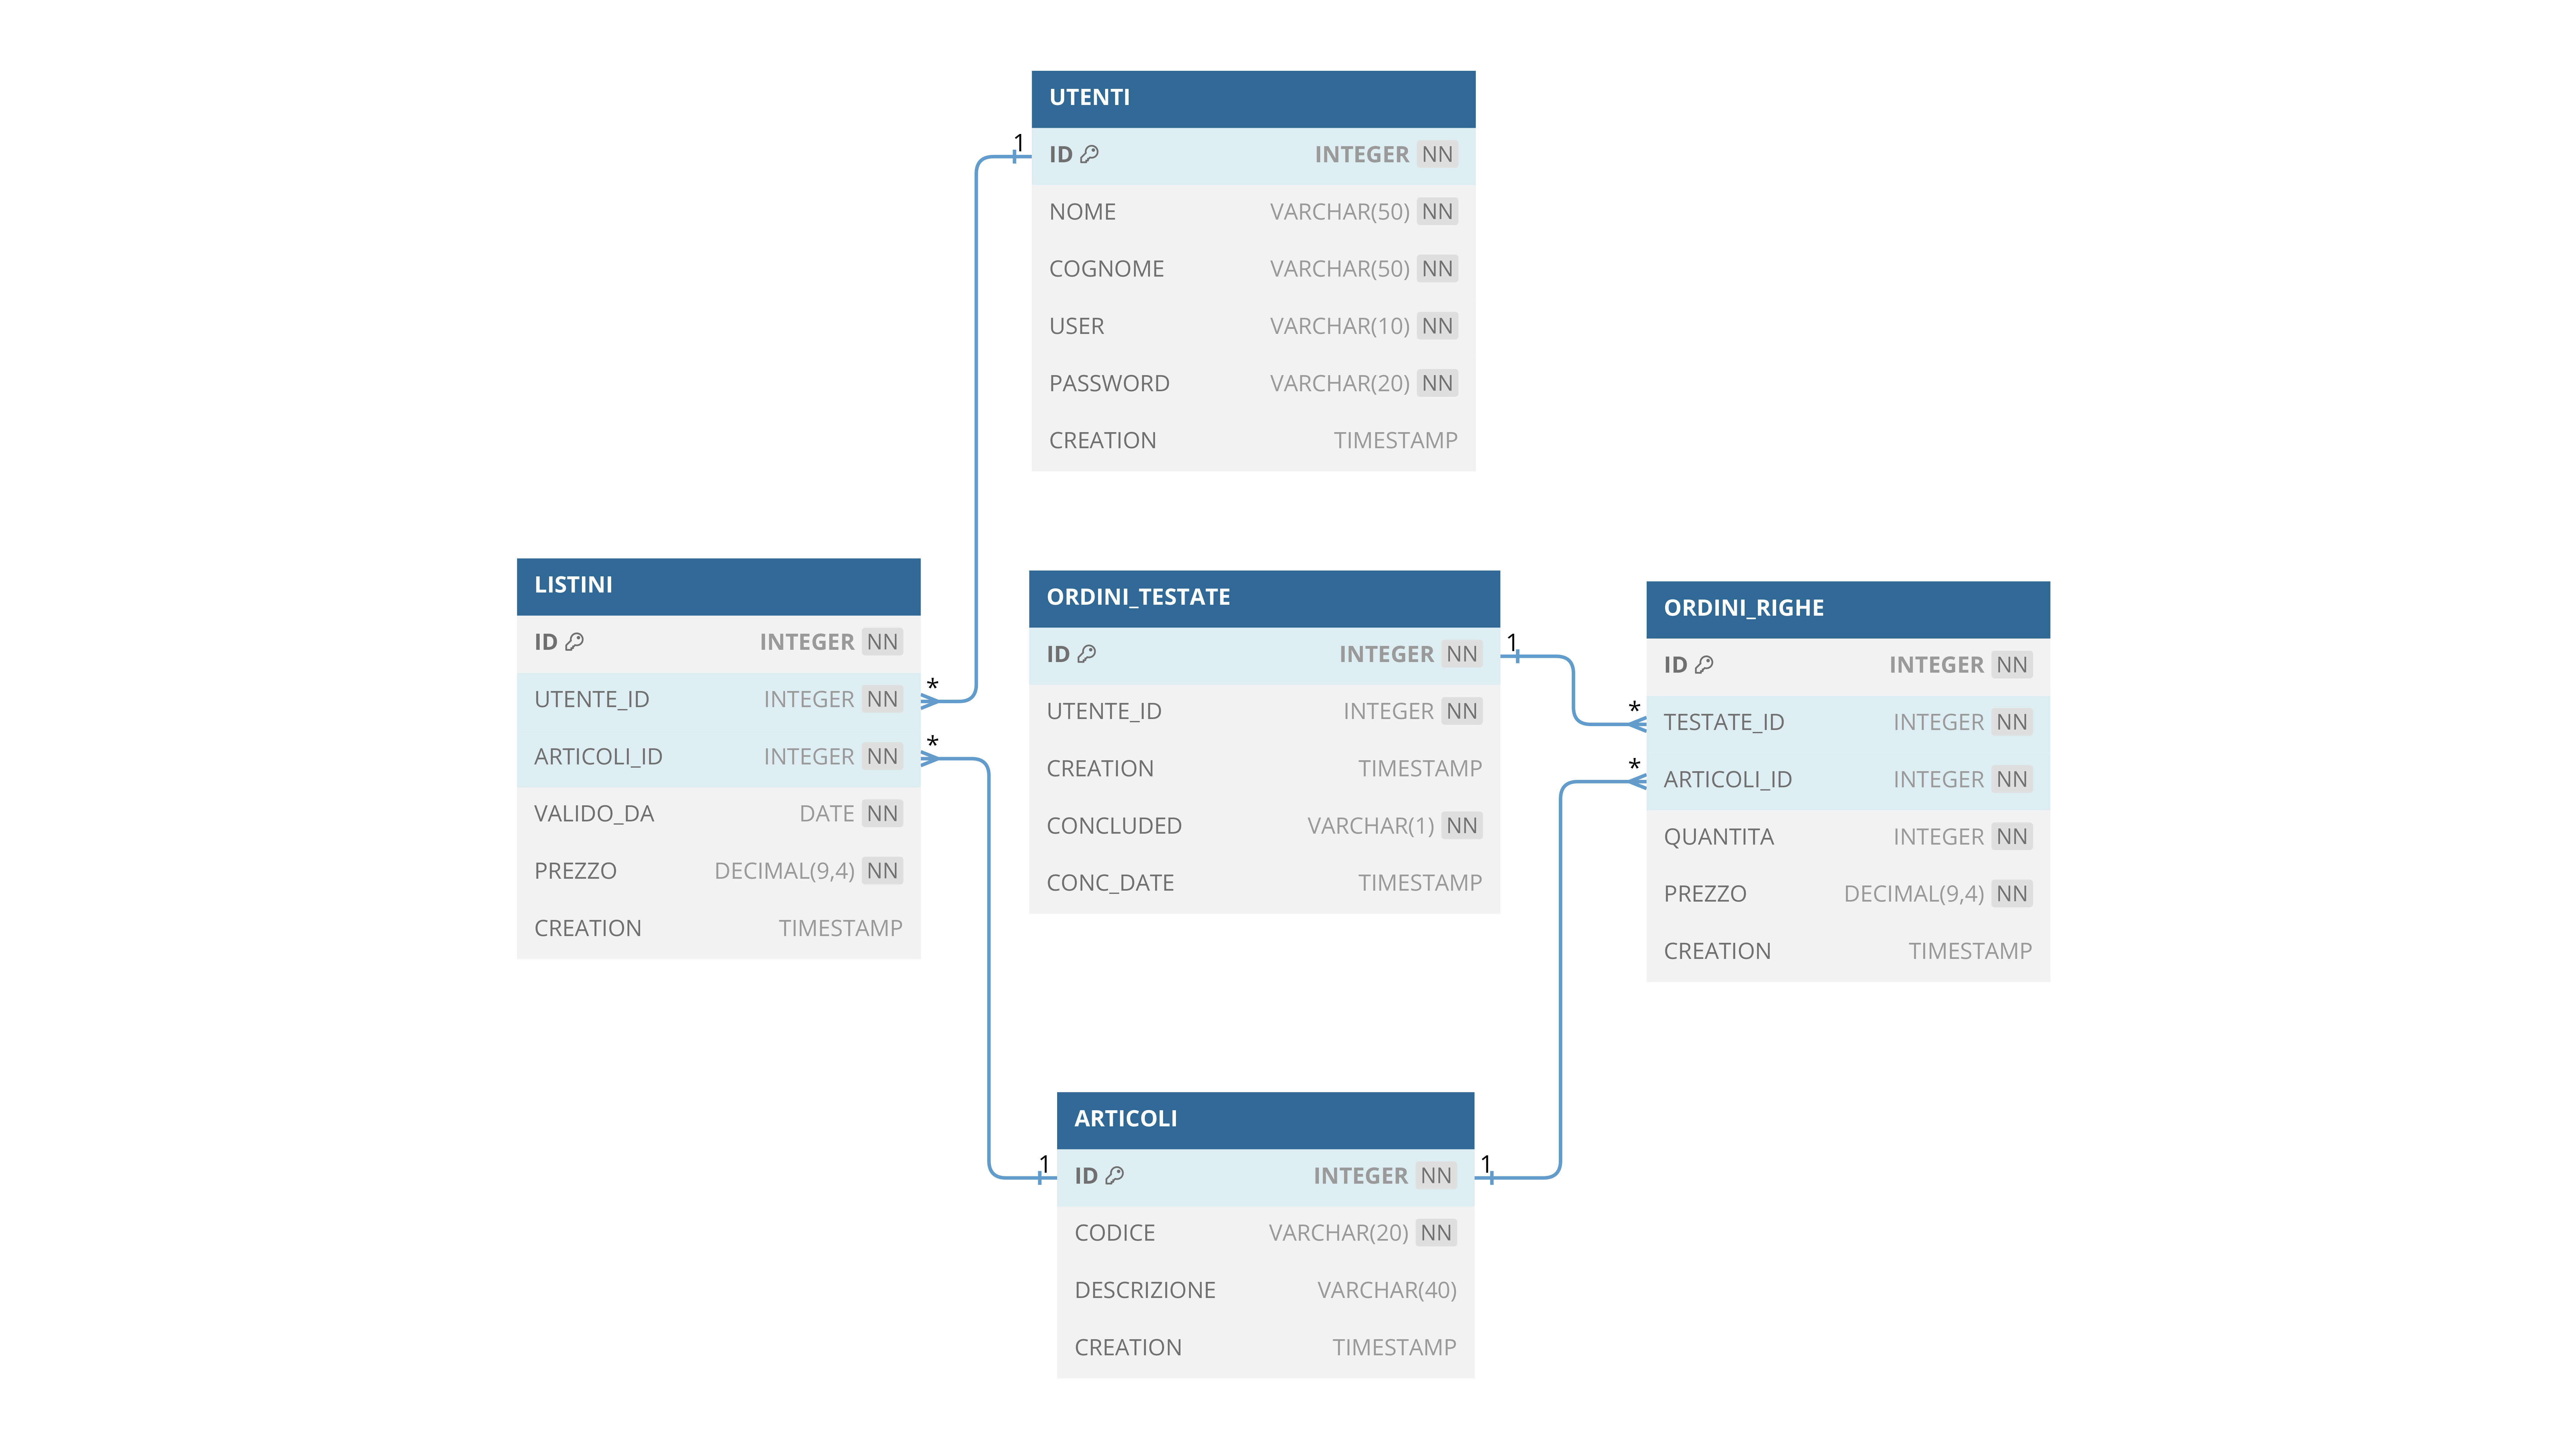
\includegraphics[width=1.6\linewidth, keepaspectratio]{Assets/dbdiagram.png}}
	\caption{Struttura del Database}
	\label{fig:dbdiagram}
\end{figure}

Nel diagramma illustrato in \Cref{fig:dbdiagram}, sono rappresentate le tabelle che costituiscono il Database, corredate delle rispettive chiavi esterne e primarie.\\
Particolarmente rilevante è la relazione tra le tabelle "UTENTI" e "ARTICOLI", che è di tipo molti-a-molti. Tale scelta deriva dalla necessità di assegnare un listino prezzi dedicato a ciascun cliente. Di conseguenza, un singolo utente può disporre di una pluralità di articoli con prezzi specifici, mentre un articolo può essere dedicato a numerosi utenti. Questo meccanismo permette di personalizzare l'esperienza dell'utente, fornendo tariffe e condizioni di vendita mirate.\\
La tabella "LISTINI" rappresenta l'insieme dei prezzi per prodotto dedicato a ciascun utente, di fatto tale approccio favorisce una gestione flessibile dei costi e promuove una maggiore adattabilità commerciale, consentendo di offrire politiche di prezzo diversificate.\\
Ulteriori relazioni rilevanti sono quelle tra le tabelle "ARTICOLI" e "ORDINI\_TESTATE". La relazione molti-a-molti tra queste due entità riflette la possibilità che un articolo possa essere acquistato da più utenti diversi (in sostanza che un articolo possa stare in più "carrelli"). D'altra parte, la tabella "ORDINI\_TESTATE" consente di raggruppare diversi articoli o prodotti all'interno di un singolo ordine. Ciò significa che un ordine può contenere una molteplicità di articoli, ognuno con la propria quantità e prezzo specifico (tutto questo salvato nella tabella ORDINI\_RIGHE), che viene ottenuto dalla tabella "LISTINI" come scritto in precedenza. In sostanza, quindi, ogni prodotto che un utente acquista ha un prezzo specifico dalla tabella LISTINI: quando il prodotto viene aggiunto al carrello, viene registrato nella tabella ORDINI\_RIGHE e il riferimento al carrello appena creato viene memorizzato nella tabella ORDINI\_TESTATE.

\subsubsection{Query}
Le query utilizzate per interrogare il Database possono variare a seconda della richiesta ricevuta. Durante la fase di login, il Client invia al Server sia lo username che la password inseriti dall'utente nell'applicazione, e di conseguenza, diventa indispensabile confrontare tali informazioni con quelle memorizzate nel Database. A tal fine, si impiega la seguente query:
\begin{lstlisting}[language=sql] [H]
	SELECT u.ID FROM UTENTI u 
	WHERE u.USER = 'user' AND u.PASSWORD = 'password'
\end{lstlisting}

\noindent
Una volta effettuato il login, l'utente ha la possibilità di ricercare prodotti attraverso l'apposita barra di ricerca. A tale scopo, il Client invia una richiesta specifica al Server contenente la parola chiave desiderata, con l'obiettivo di ottenere i prodotti corrispondenti e relativo prezzo. La risposta fornita dal Server, quindi, consiste in una lista di prodotti il cui nome contiene la parola chiave indicata, accompagnata dal relativo prezzo dedicato all'utente.\\
\\
Per effettuare questa operazione, viene utilizzata la seguente query:
\begin{lstlisting}[language=sql] [H]
	SELECT l.ARTICOLI_ID, a.DESCRIZIONE, l.PREZZO FROM UTENTI u
	INNER JOIN LISTINI l ON u.ID = l.UTENTE_ID
	INNER JOIN ARTICOLI a ON l.ARTICOLI_ID = a.ID 
	AND u.ID = id AND LOWER(a.DESCRIZIONE) LIKE '%keyword%'
\end{lstlisting}

\noindent
Per esempio, un possibile output ricercando la keyword "mele" è il seguente:
\begin{lstlisting}[language=json] [H]
	{
		"body":[
		{
			"id":1341,
			"name":"MELE RED DELIC 19K",
			"price":0.028,
			"quantity":0
		},
		{
			"id":1387,
			"name":"MELE RED DELIC 18K",
			"price":0.028,
			"quantity":0
		},
		{
			"id":1697,
			"name":"MELE RED DELIC 12K",
			"price":0.028,
			"quantity":0
		}
		]
	}
\end{lstlisting}

\noindent
Una volta individuato il prodotto desiderato, l'utente ha la possibilità di aggiungerlo al carrello mediante la creazione di una testata. Per compiere questa operazione, il Client invia una richiesta specifica al Server contenente il codice del prodotto e la quantità relativa (impostata di default a 1).
Successivamente, il Server verifica se il Client ha specificato la testata nell'header; nel caso in cui non sia stata specificata, il sistema procede a crearne una corrispondente per l'utente in questione. A tal scopo, si utilizza la seguente query (con parametri testataId, prodId, orderQuantity e userId):
\begin{lstlisting}[language=sql, firstnumber=1] [H]
	INSERT INTO ORDINI_TESTATE (UTENTE_ID) 
	SELECT ID FROM UTENTI WHERE ID = userId
\end{lstlisting}

\noindent
Se invece è specificata si controlla che non sia stata chiusa, che l'ordine non sia già stato inserito e in tal caso, se ne aumenta la quantità chiudendo la richiesta.
Le query sono rispettivamente:
\begin{lstlisting}[language=sql, firstnumber=1] [H]
	SELECT CONCLUDED FROM ORDINI_TESTATE WHERE ID = testataId
	
	SELECT * FROM ORDINI_RIGHE 
	WHERE TESTATE_ID = testataId AND ARTICOLI_ID = prodId;
	
	UPDATE ORDINI_RIGHE
	SET QUANTITA = orderQuantity
	WHERE TESTATE_ID = testataId AND ARTICOLI_ID = prodId;
\end{lstlisting}

\noindent
Nel caso in cui l'ordine venga inserito per la prima volta, esso verrà aggiunto nella tabella ORDINI\_RIGHE. Durante questo processo, verrà recuperato il prezzo corrispondente dalla tabella LISTINI utilizzando la seguente query:\footref{fn1}:
\begin{lstlisting}[language=sql, firstnumber=1] [H]
	INSERT INTO ORDINI_RIGHE 
	(TESTATE_ID, ARTICOLI_ID, QUANTITA, PREZZO)
	SELECT testataId, prodId, orderQuantity, l.PREZZO 
	FROM UTENTI u
	INNER JOIN LISTINI l ON u.ID = l.UTENTE_ID
	INNER JOIN ARTICOLI a ON l.ARTICOLI_ID = a.ID 
	AND u.ID = userId AND l.ARTICOLI_ID = prodId
\end{lstlisting}

\noindent
Infine il Client può richiedere di visualizzare il carrello con gli ordini aggiunti. In tal caso la query\footref{fn1} è la seguente:
\begin{lstlisting}[language=sql, firstnumber=1] [H]
	SELECT l.ARTICOLI_ID, a.DESCRIZIONE, l.PREZZO, o.QUANTITA
	FROM LISTINI l
	INNER JOIN ARTICOLI a ON l.ARTICOLI_ID = a.ID
	INNER JOIN ORDINI_RIGHE o ON a.ID = o.ARTICOLI_ID 
	WHERE o.TESTATE_ID = testataId AND l.UTENTE_ID = userId
\end{lstlisting}

\noindent
È stata altresì introdotta la possibilità di reperire informazioni sull'account utente, nonché di cancellare ordini dal carrello, concludere e chiudere testate. Queste funzionalità vengono gestite attraverso query semplici e di facile comprensione del tipo SELECT, UPDATE e DELETE, quindi evito di riportarle qui per risparmiare il lettore da una lettura superflua. L'unico accenno che mi sento di dare è sulla chiusura di una testata, la quale è possibile farla impostando ad 1 il campo CONCLUDED della tabella ORDINI\_TESTATE (immagine \ref{fig:dbdiagram}).

\subsection{Token: Come vengono generati e usati} \label{section_token}
Durante il ciclo di vita del Server, in determinati momenti, diventa essenziale acquisire l'id dell'utente che ha effettuato la richiesta, al fine di gestirla nel modo più adeguato. Di fatto, le query menzionate in precedenza impiegano ampiamente l'identificativo dell'utente (userId). Tuttavia, per motivi di sicurezza, questo "id" non può essere trasmesso tramite l'URI. Un primo approccio, quindi, che solitamente viene utilizzato quando si devono gestire degli utenti è tenere sul Server le informazioni necessarie, lette inizialmente dal Database, in una cache (solitamente rappresentata da una Map, nel mio caso una Map dove la chiave è il token e il valore è l'id utente) e interrogarla ogni qual volta sia necessario avere dati specifici. Tuttavia, questa metodologia può causare problemi di efficienza poiché la memorizzazione di tutte queste informazioni, per ciascun utente, può comportare un notevole aumento nell'utilizzo delle risorse e conseguentemente rallentare l'intero sistema in modo esponenziale.\\
I token JWT sono stati quindi pensati appositamente per rendere l'applicazione scalabile, facendo in modo che siano gli utenti a persistere sui loro dispositivi i dati necessari, affinché le loro richieste vengano gestite nella maniera più corretta. Grazie a questo approccio, non è più necessario utilizzare una cache sul Server, consentendo di liberare risorse e semplificare il mantenimento del Server.
Come descritto nel \Cref{subsub:secure}, la creazione dei token richiede l'utilizzo di una chiave simmetrica, usata per criptare i token JWT; la chiave e i token vengono quindi creati nel seguente modo:
\begin{lstlisting}[language=Java, firstnumber=1][H]
	
	/* Creazione della chiave */
	Key secretKey = Keys.secretKeyFor(SignatureAlgorithm.HS256);
	
	/* Metodo che genera un token firmato */
	public String generateToken(int userId) {
		return Jwts.builder()
		.setSubject(String.valueOf(userId))
		.setIssuer(ISSUER)
		.signWith(secretKey)
		.compact();
	}
\end{lstlisting}
\noindent
Durante la fase di accesso, l'id  dell'utente viene quindi estratto dal Database, inserito nel token JWT e, nei successivi invii di richieste, quest'identificatore verrà recuperato direttamente dal token, eliminando la necessità di consultare una cache.\\
Al fine di garantire l'autenticità e l'integrità dei token, evitando potenziali manomissioni da parte di Client malevoli, il Server adotta un metodo di verifica della firma del token mediante l'utilizzo della propria chiave simmetrica. Questo processo permette al Server di assicurarsi che il token sia valido e provenga da una fonte attendibile (cioè lui stesso!). Il metodo di verifica è il seguente:
\begin{lstlisting}[language=Java][H]
	/* Ritorna true se il token e' stato creato con secretKey, false altrimenti */
	public boolean isValid(String token) {
		try {
			Jwts.parserBuilder()
			.setSigningKey(secretKey)
			.requireIssuer(ISSUER)
			.setAllowedClockSkewSeconds(CLOCK_SKEW_SECONDS)
			.build()
			.parseClaimsJws(token);
			return true;
		}catch (JwtException e) {
			return false;
		}
	}
\end{lstlisting}

\noindent
Per verificare invece la sola scadenza del token, viene utilizzato il seguente metodo:
\begin{lstlisting}[language=Java][H]
	// Ritorna true se il token e' scaduto, false altrimenti
	public boolean isExpired(String token) {
		try {
			DecodedJWT jwt = JWT.decode(token);
			Date expirationDate = jwt.getExpiresAt();
			Date now = new Date();
			
			Calendar calendar = Calendar.getInstance();
			calendar.setTime(expirationDate);
			calendar.add(Calendar.SECOND, CLOCK_SKEW_SECONDS);
			expirationDate = calendar.getTime();
			
			return expirationDate.before(now);
		} catch (Exception e) {
			return true;
		}
	}
\end{lstlisting}

\noindent
E' facile intuire che questa chiave deve essere salvata da qualche parte al momento della sua creazione, in quanto la perdita di essa (per esempio al riavvio del Server) invaliderebbe tutti i token inviati ai Client, obbligandoli ad eseguire nuovamente il login.

\subsubsection{Creazione chiave e persistenza su disco} \label{subsub:key_creation_and_disk_persistency}
Per generare la chiave simmetrica viene impiegata la classe Keys della libreria JsonWebToken (vedi \Cref{sub:jwt}) nel seguente modo:
\begin{lstlisting}[language=Java, firstnumber=1][H]
	private Key generateKey() {
		return Keys.secretKeyFor(SignatureAlgorithm.HS256);
	}
\end{lstlisting}

\noindent
Tuttavia si è ritenuto poco sicuro salvarla semplicemente sul disco utlizzando la Serializzazione\cite{serializable} (essendo l'oggetto Key serializzabile) fornita da Java, quindi è stato deciso di criptarla mediante l'utilizzo di un altra chiave e scrivendone poi i byte cifrati sul disco rigido del Server. Per generare questa seconda chiave è necessario tuttavia avere una password, che di default ha valore pre-settato essendo in scopi didattici ma, in casi più normali, si sarebbe ad esempio chiesta all'avvio del Server o salvata su qualche disco sicuro.
Il procedimento è quindi:
\begin{enumerate}
	\item Convertire la password da tipo String a SecretKey
	\begin{lstlisting}[language=Java, firstnumber=1][H]
private SecretKey getPasswordKey(String password) {
	try {
		byte[] key = 
		password.getBytes(StandardCharsets.UTF_8);
				
		MessageDigest md = MessageDigest.getInstance("SHA-256");
				
		key = md.digest(key);
		return new SecretKeySpec(key, "AES");
				
	} catch (NoSuchAlgorithmException e) {
		e.printStackTrace();
	}
			
	throw new Exception("password exception");
}
	\end{lstlisting}
	
	\item Usare la SecretKey definita nel punto 1. per reperire la chiave dal disco. Il metodo definito sotto ritorna "null" in caso non esista alcuna chiave sul disco, o la Key in caso questa si trovi nella cartella definita dalla variabile globale "KEY\_PATH"
	\begin{lstlisting}[language=Java][H]
private Key readKeyFromFile(SecretKey passwordKey) {
	Path path = Path.of(KEY_PATH);
	if(Files.exists(path)) {
		byte[] encryptedMsg = Files.readAllBytes(path);
		
		byte[] decrypted = 
		decrypt(encryptedMsg, passwordKey);
		
		// Crea una nuova Key usando l'algoritmo HMAC-SHA
		return Keys.hmacShaKeyFor(decrypted);
	}
	
	return null;
}

byte[] decrypt(byte[] message, SecretKey passwordKey) {
	try {
		Cipher cipher = 
		Cipher.getInstance("AES/ECB/PKCS5PADDING");
		
		cipher.init(Cipher.DECRYPT_MODE, passwordKey);
		return cipher.doFinal(message);
	} catch (Exception e) {
		e.printStackTrace();
	}
	
	throw new Exception("Error while decrypting");
}
	\end{lstlisting}
	\item Se questa non è presente ne genero una nuova, ne vengono cifrati i byte usando la password e infine salvato il risultato sul disco
	\begin{lstlisting}[language=Java][H]
		Key secretKey = generateKey();
		
		private void writeKeyToFile(SecretKey passwordKey) 
		throws Exception {
			byte[] message = secretKey.getEncoded();
			
			byte[] encryptedMsg = encrypt(message, passwordKey);
			Files.write(Path.of(KEY_PATH), encryptedMsg);
		}
		
		private byte[] encrypt(byte[] message, SecretKey passwordKey) 
		throws Exception {
			try {
				Cipher cipher = 
				Cipher.getInstance("AES/ECB/PKCS5Padding");
				
				cipher.init(Cipher.ENCRYPT_MODE, passwordKey);
				return cipher.doFinal(message);
			} catch (Exception e) {
				e.printStackTrace();
			}
			
			throw new Exception("Error while crypting");
		}
		
	\end{lstlisting}
	
	\item Al riavvio del Server, ripartire dal punto numero 1
\end{enumerate}


\newpage
\noindent
Tutto questo si può riassumere quindi in:
\begin{lstlisting}[language=Java][H]
	SecretKey passwordKey = getPasswordKey(password);
	Key secretKey = readKeyFromFile(passwordKey);
	
	if (secretKey == null) {
		secretKey = generateKey();
		
		writeKeyToFile(passwordKey);
	}
\end{lstlisting}

\noindent
Più nello specifico, per generare la chiave dalla password viene ottenuta un'istanza dell'algoritmo hash SHA-256 attraverso la classe MessageDigest. SHA-256 è una funzione di hashing crittografica che restituisce un valore hash di 256 bit.\\
Per la criptazione e decriptazione viene usata la classe Cipher della libreria standard di Java, la quale viene impostata in modo che vengano usati gli algoritmi di AES, ECB e PKCS5Padding come descritto nella \Cref{subsub:secure}.

\subsection{Comunicare con il Server e Gestione delle\\ richieste tramite Javalin}\label{subsub:javalin}
Come descritto nella \Cref{section1}, il Server è stato implementato mediante l'utilizzo del framework Javalin il quale, al momento dell'avvio, crea un'istanza della classe Javalin utilizzando una porta predefinita, secondo queste modalità:
\begin{lstlisting}[language=Java, firstnumber=1][H]
	Javalin app = Javalin.create().start(7777);
\end{lstlisting}


\noindent
In seguito, si procede alla definizione delle rotte dell'applicazione: queste rappresentano gli endpoint del Server che successivamente si definiranno tramite delle URI. Le rotte vengono specificate mediante l'uso dei metodi HTTP come GET, POST, DELETE, eccetera, e richiedono l'inserimento di una callback (con un parametro context di tipo Context per eseguire diverse azioni, tra cui parsing del path o accesso all header) che verrà invocata quando un Client eseguirà una richiesta HTTP verso quella specifica route. Nel contesto di Javalin, per creare una route, ad esempio una route di tipo GET, si utilizza la seguente sintassi:

\begin{lstlisting}[language=Java]
	context.get("uri", context -> {
		// gestione della richiesta..
	});
\end{lstlisting}

\noindent
Per definire una route che richiede un parametro, si utilizza invece il seguente approccio:
\begin{lstlisting}[language=Java]
	context.get("/{param}", context -> {
		String value = context.pathParam("param");
		// gestisci la richiesta usando value..
	});
\end{lstlisting}

\noindent
In sostanza le routes costituiscono il meccanismo chiave per consentire l'interazione tra il Server e i Client.
Nel mio caso quindi le rotte sono le seguenti:
\begin{lstlisting}[language=Java, firstnumber=5][H]
	app.get("/users/login/{username}={password}", context -> {})
	app.get("/users/profile", context -> {})
	app.get("/users/logout", context -> {})
	app.get("/search/desc={desc}", context -> {})
	app.get("/search/code={code}", context -> {})
	app.get("/testata/{tid}", context -> {})
	app.get("/testata/{tid}/cart", context -> {})
	app.post("/orders/add={pid}&quantity={qt}", context -> {})
	app.post("/orders/add={pid}", context -> {})
	app.post("/orders/quantity/{pid}={q}", context -> {})
	app.post("/orders/complete", context -> {})
	app.delete("/orders/remove={pid}", context -> {})
\end{lstlisting}
\noindent
Il meccanismo di gestione delle richieste si basa quindi sull'estrapolare i valori passati come parametri dall'URI, costruire una query in base alla natura della richiesta (come descritto nella \Cref{section2}), ed eseguire tale query per ottenere i dati desiderati. Il Server risponderà al Client restituendo un oggetto JSON contenente il risultato ottenuto o un messaggio di errore in caso di problematiche.
È fondamentale notare che la maggior parte delle richieste deve includere il token di accesso (per ottenere l'ID utente, come illustrato nella \Cref{section_token}), e in alcuni casi, potrebbe essere richiesto anche l'ID della testata (ad esempio, quando si intende aggiungere un prodotto al carrello, come dettagliato nella \Cref{section2}).

\subsubsection{Messaggi di errore}
Durante il ciclo di vita dell'applicazione, può capitare che il Server debba restituire messaggi di errore: questi messaggi sono sempre in JSON e seguono il seguente formato:
\begin{lstlisting}[language=JSON, firstnumber=1][H]
	{
		"code": codice numerico rappresentativo dell'errore,
		"message": "Messaggio testuale esplicativo del codice"
	}
\end{lstlisting}
\section{Client}
Il Client è stato implementato utilizzando il linguaggio di programmazione Dart e si basa sul framework Flutter di Google. All'avvio dell'applicazione vengono caricati dal disco la testata corrente e i token utente, se disponibili. Successivamente, viene verificato se l'utente ha già effettuato l'accesso, basandosi sulla presenza di tali token: in caso positivo, l'app restituirà la pagina Home; in caso contrario, la prima schermata visualizzata sarà quella di Login. Nel corso di questa fase di inizializzazione, si controlla anche la validità del token di aggiornamento: nel caso in cui risulti scaduto, l'utente riceverà un avviso dialog informando che la sessione è scaduta e che dovrà effettuare nuovamente l'accesso per ottenere un nuovo token di aggiornamento. Come vedremo più avanti, in questa fase vengono anche creati tutti i Provider necessari alla comunicazione tra Widget e il caricamento del carrello salvato localmente.\\
Infine il processo di progettazione e sviluppo del Client si articola in tre macro categorie: la fase di disegno dell'app attraverso l'utilizzo di Figma, la successiva trasposizione di tale progettazione all'interno di Flutter e, per  ultimo, l'implementazione concreta delle funzionalità dell'applicazione.

\subsection{Mockup dell'Applicazione}
Il mockup dell'applicazione è stato realizzato utilizzando Figma e corrisponde a 4 schermate principali: Login, Home, Carrello e Profilo. La navigazione all'interno dell'app è stata implementata tramite la libreria "go\_router" (vedi \Cref{subsub:go_router}) ed è stata progettata in modo che l'utente possa sempre tornare indietro, fintanto che è possibile, al fine di garantire un'esperienza fluida e continuativa.

\begin{figure}[h]
	\centering
	\begin{tikzpicture}[node distance=5cm, auto]
		% Definizione dei nodi
		\node[circle, draw] (Login) {Login};
		\node[circle, draw, right of=Login] (Home) {Home};
		\node[circle, draw, right of=Home] (Carrello) {Carrello};
		\node[circle, draw, below of=Home] (Profilo) {Profilo};
		
		% Collegamenti
		\draw[->, shorten >=5pt, shorten <=5pt] (Login) -- (Home);
		\draw[<->, shorten >=5pt, shorten <=5pt] (Home) -- (Carrello);
		\draw[<->, shorten >=5pt, shorten <=5pt] (Home) -- (Profilo);
		
		\draw[->, shorten >=5pt, shorten <=5pt] (Home) to[out=-160, in=-10] node[midway, below] {in caso di logout} (Login);
	\end{tikzpicture}
	\caption{Schema di navigazione tra le schermate}
\end{figure}

\def\ImageSize{0.35}
 
\subsubsection{Login}
La pagina di Login costituisce il punto di accesso che l'utente incontra al primo avvio dell'applicativo (o in seguito a una fase di logout). Essa è caratterizzata da una colonna contenente due campi di testo e un pulsante dedicato all'invio dei dati.
\begin{figure}[H]
    \centering
    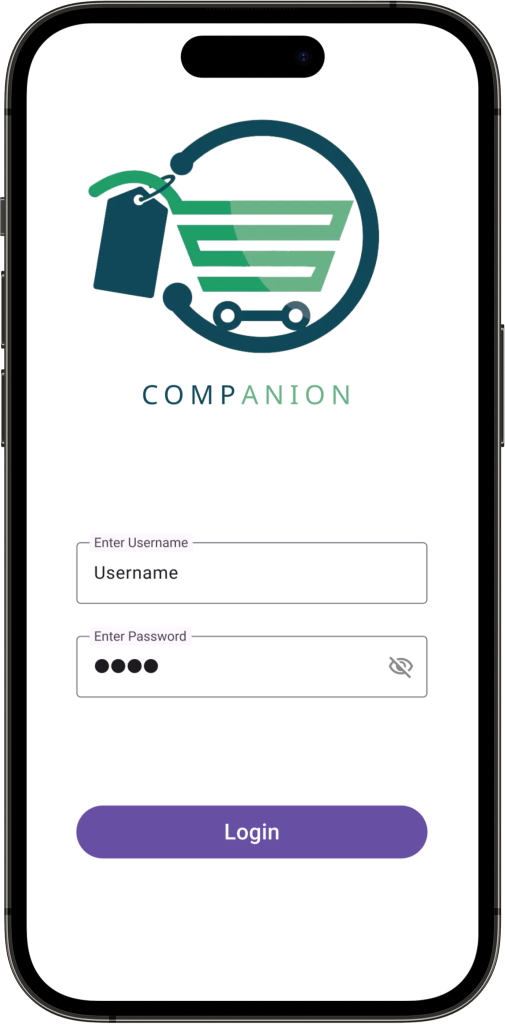
\includegraphics[width=\ImageSize\linewidth]{Assets/Login mockup.png}
    \caption{Pagina di Login}
    \label{login_figma}
\end{figure}
\noindent

\newpage
\subsubsection{Home}
La schermata Home è la pagina principale che compare quando si è eseguito il login. Come richiesto dal tutor aziendale è caratterizzata da una barra di ricerca, che contiene al suo interno anche un pulsante per aprire il Drawer, una lista con i prodotti ricercati e un pulsante per andare alla pagina del carrello. Le Card \cite{card} della lista sono composte da un immagine facoltativa (a seconda se il Server la rende disponibile o meno), del testo che descrive il prodotto con relativo codice e un pulsante adibito all'aggiunta nel carrello. L'immagine di sfondo compare in caso di lista vuota ed è stata inserita a scopo di riempimento.
\begin{figure}[h]
\centering
	\begin{minipage}[t]{\ImageSize\linewidth}
		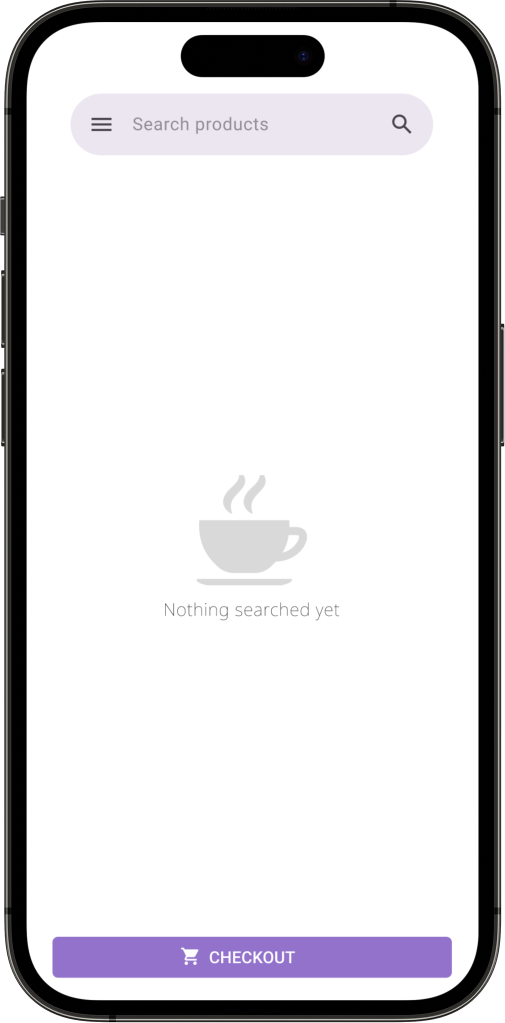
\includegraphics[width=\linewidth]{"Assets/Empty mockup.png"}
		\caption{Pagina Home con ricerca}
		\label{fig:figma_home}
	\end{minipage}
	\hspace{1em}
	\begin{minipage}[t]{\ImageSize\linewidth}
		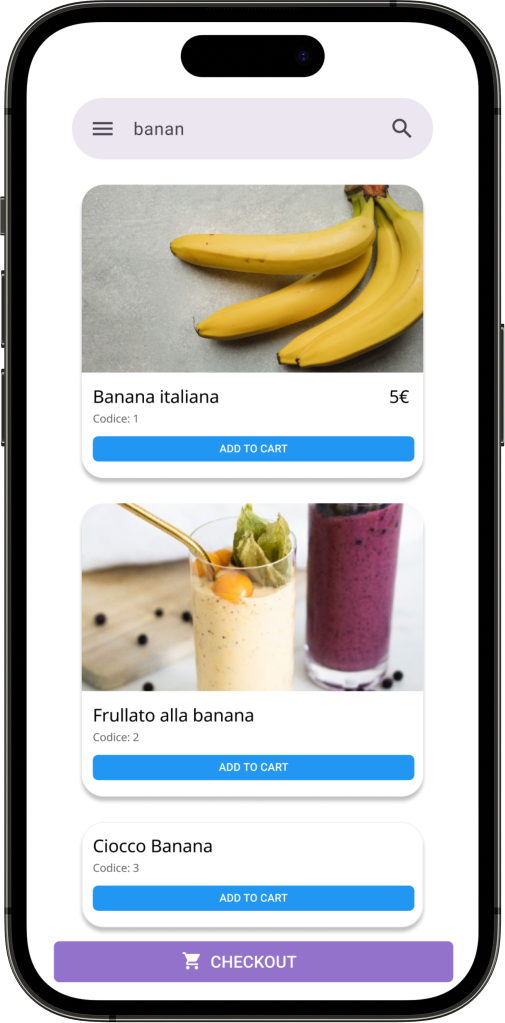
\includegraphics[width=\linewidth]{"Assets/List mockup.png"}
	\end{minipage}

\end{figure}

\newpage
\subsubsection{Carrello}
La pagina del carrello presenta anch'essa una disposizione in forma di lista e, in conformità alle direttive dettate dal mio supervisore aziendale, ogni Card di essa offre la possibilità di modificare la quantità di ciascun articolo tramite specifici pulsanti, consentendo inoltre di eliminare ogni singolo elemento dal carrello mediante uno swipe verso sinistra. Si provvede altresì a indicare il prezzo unitario di ciascun prodotto insieme all'importo totale corrispondente alla quantità selezionata. Infine, nella parte inferiore della pagina, è presente un pulsante dedicato all'invio dell'ordine, accompagnato dal riepilogo del prezzo totale.
\begin{figure}[H]
    \centering
    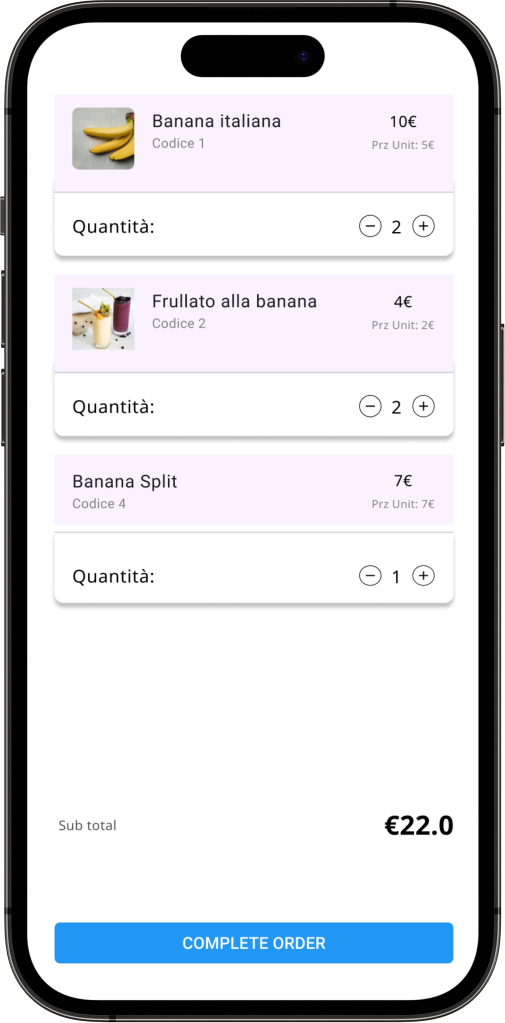
\includegraphics[width=\ImageSize\linewidth]{Assets/Cart mockup.png}
    \caption{Pagina del Carrello}
    \label{fig:figma_cart}
\end{figure}

\newpage
\subsubsection{Profilo}
La pagina del profilo è stata creata per mostrare le informazioni dell'utente. Avendo a disposizione di pochi dati da mostrare, ho deciso di optare per una soluzione a "lista" che mostra giusto le informazioni essenziali spezzando il più possibile a fini di riempimento (per esempio la divisione tra nome e cognome in 2 campi di testo diversi è voluta)
\begin{figure}[H]
\centering
	\begin{minipage}[t]{\ImageSize\linewidth}
		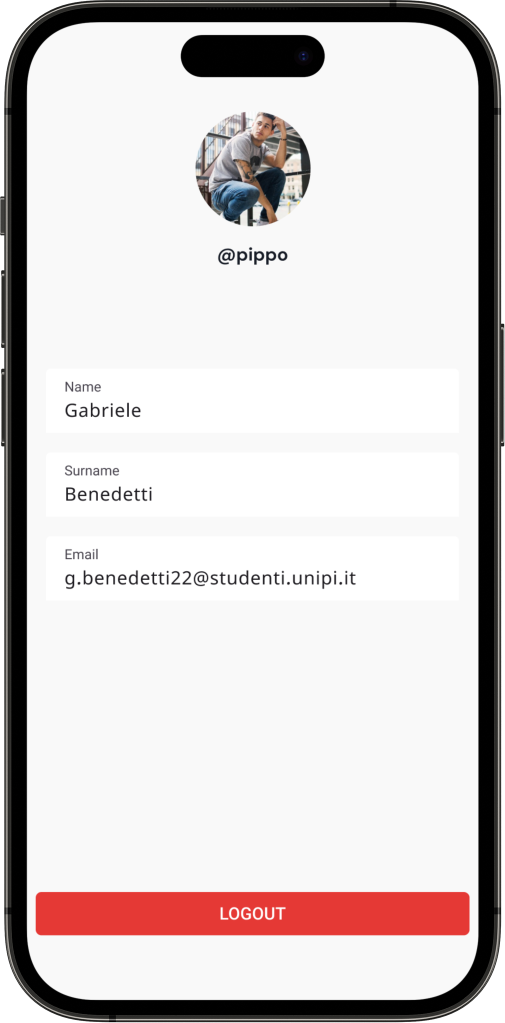
\includegraphics[width=\linewidth]{"Assets/mockup image.png"}
	\end{minipage}
	\hspace{1em}
	\begin{minipage}[t]{\ImageSize\linewidth}
		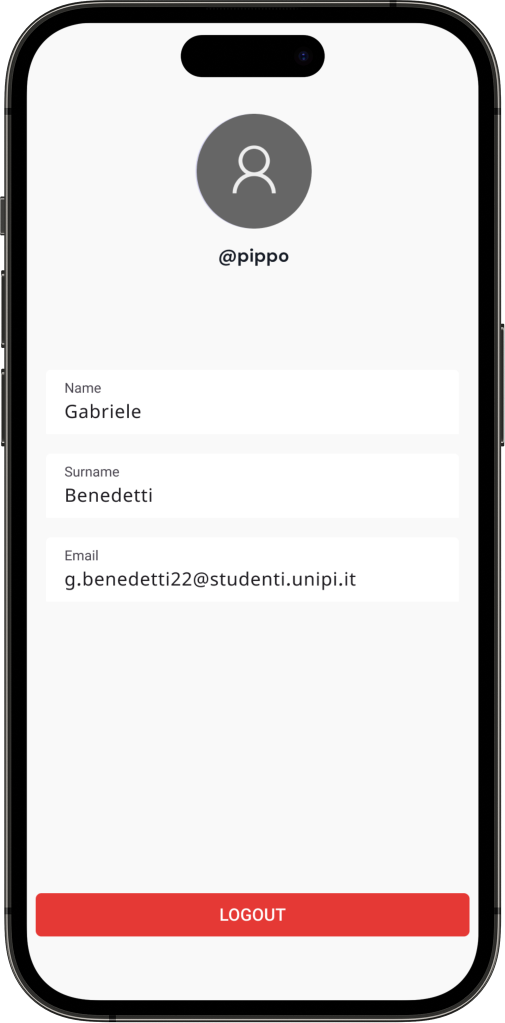
\includegraphics[width=\linewidth]{"Assets/mockup no image.png"}
	\end{minipage}
	\captionof{figure}{Pagina del Profilo utente}
	\label{fig:figma_profile}
\end{figure}


\subsection{Da Figma a Flutter - Sviluppo della UI}
Tutte le schermate dell'applicazione sono state inserite dentro uno Scaffold. L'AppBar inclusa è comune a tutte le schermate, contenente un titolo e una barra di caricamento richiamabile mediante Provider (vedi \Cref{lab_widget_communication}).\\
Nelle sezioni successive verrà menzionato notevolmente anche il Widget Expanded, quindi il lettore è richiamato a rileggere la \Cref{subsub:expanded} in caso non si abbia chiaro a cosa serva questo Widget.
Infine vorrei sottolineare che i frammenti di codice inseriti sono da considerarsi più come strumento per capire la logica adottata dietro la costruzione dell'interfaccia, infatti molte cose verranno tralasciate poiché considerate irrilevanti.

\subsubsection{Login}
In accordo con quanto stabilito nella \Cref{login_figma}, la pagina di Login deve contenere un immagine, 2 campi di testo e un pulsante per inoltrare la richiesta di accesso.
Essendo a tutti gli effetti un form è stato quindi usata la classe Form che Flutter mette a disposizione: questo Widget permette la validazione dei campi tramite callbacks\footnote{una funzione che viene passata come parametro e poi eseguita in seguito} e l'uso di TextFormField che incorporano dei messaggi di errore in caso l'utente inserisca dei dati sbagliati. Di seguito lo pseudo-codice:
\begin{lstlisting}[language=Java, firstnumber=1][H]
TextEditingController usernameController, passwordController;
GlobalKey<FormState> formKey;

Column(
	children: [
		Expanded (
			child : Image.asset("logo.png"),
		),
		Expanded(
			child : Form(
				key : formKey, // per tenere un riferimento al form
				child : Column(
					children : [
						TextFormField(
							controller: usernameController,
						),
						TextFormField(
							controller: passwordController
						)
					]
				)
			)
		),
		Expanded(
			child : ElevatedButton(
				onPressed : () {
					String username = usernameController.text;
					String password = passwordController.text;
					login(username, password);
				},
				child : Text("Login"),
			)
		),
	],
)
\end{lstlisting}
A questo punto i dati del Form devono avere una qualche "regola di verifica" quando l'utente preme il pulsante di autenticazione. Per farlo, possiamo quindi passare una "callback" all'oggetto "TextFormField" e questa callback avrà, come parametro la stringa presente nel campo di testo e deve restituire "null" se tutto è corretto, altrimenti un messaggio di errore che verrà mostrato all'utente nel corrispettivo TextFormField. Il codice deve essere quindi modificato secondo quanto segue:
\begin{lstlisting}[language=Java, firstnumber=9][H]
child : Form(
	key : formKey,
	child : Column(
		children : [
			TextFormField(
				controller: usernameController,
				validator: (value) => isUsernameValid(value),
			),
			TextFormField(
				controller: passwordController,
				validator: (value) => isPasswordValid(value),
			)
		]
	)
)

// ritorna null se username e' ok, il messaggio di errore altrimenti
String? isUsernameValid(String? username) {
	if (username == null) 
	 return "Username cannot be null";
	 
	if (username.trim().isEmpty)
	 return "Username cannot be empty";
	 
	if (username.isEmpty)
	 return "Username cannot be only whitespaces";
	 
	if (username.contains(" "))
	 return "Username can't contain spaces";
	
	return null;
}

// ritorna null se password e' ok, il messaggio di errore altrimenti
String? isPasswordValid(String? password) {
	if (password == null)
	 return "Password cannot be null";
	 
	if (password.isEmpty)
	 return "Password cannot be empty";
	 
	if (password.trim().isEmpty)
	 return "Password cannot be only whitespaces";
	
	return null;
}
\end{lstlisting}

\noindent
Infine, per effettuare effettivamente la convalida del form, sarà necessario implementare la funzione di login. Basterà tuttavia chiamare il metodo "validate()", tramite la formKey definita globalmente, che attiverà le callback descritte prima e poi restituirà "true" se i dati sono validi, "false" altrimenti.\\ In codice:
\begin{lstlisting}[language=Java, firstnumber=1][H]
	void login(String username, String password) async {
		if (formKey.currentState!.validate()) {
			// form valido
		}
	}
\end{lstlisting}

\noindent
\subsubsection{Home} \label{subsub:home}
In accordo con quanto mostrato in \Cref{fig:figma_home} la pagina Home consiste in una SearchBar, che l'utente può usare per ricercare i prodotti e aprire il Drawer, una lista e un pulsante per andare alla pagina del carrello (di cui non approfondirò essendo un semplice pulsante con applicato dello stile). Questi 3 componenti sono stati sviluppati separatamente e inclusi all'interno di un Widget Column\footnote{Widget Flutter per disporre gli elementi in modo verticale} affinché stiano uno sotto l'altro. In codice:
\begin{lstlisting}[language=Java, firstnumber=1][H]
Column (
	children : [
		CompanionSearchBar(),
		ProductsList(),
		GotoCartButton()
	]
)
\end{lstlisting}

\newpage
\paragraph{CompanionSearchBar}

\noindent
Come è facile intuire dal nome, la SearchBar è stata ricreata da zero utilizzando un TextField standard, invece di impiegare il Widget di base fornito da Flutter: questo perchè la SearchBar nativa non fornisce la possibilità di passare una callback richiamabile quando l'utente preme il pulsante di invio sulla tastiera (fisica o virtuale), bensì è presente la sola possibilità di inserire una callback quando l'utente immette un qualsiasi carattere alfa-numerico o carattere speciale. Questa mancanza non mi ha permesso di poter gestire adeguatamente la ricerca dei prodotti, soprattutto a livello di efficienza in quanto eseguire una richiesta per carattere immesso richiede un uso sconsiderato delle risorse.\\
La CompanionSearchBar è dotata di un Hamburger menù richiamabile mediante l'apposita icona di prefisso e un ulteriore icona di suffisso che cambia in base a se l'utente sta scrivendo oppure no: se è presente del testo allora l'icona sarà funzionale e di pulitura (cioè l'utente può cliccarci per pulire il TextField) altrimenti viene mostrata l'icona base di ricerca che è fittizia. Questa implementazione non è nel mockup ed è stata decisa in fase di sviluppo per richiamare l'esperienza offerta dalle app mobile simili più famose, garantendo un senso di familiarità agli utenti. In codice:
\begin{lstlisting}[language=Java, firstnumber=1][H]
TextEditingController controller = TextEditingController();
bool isTyping = false;

TextField(
	controller: controller,
	textInputAction: TextInputAction.search,
	onSubmitted: (value) {
		setState(() {
			isTyping = false;
			// se sono presenti solo spazi bianchi
			if (value.trim().isEmpty) {
				return;
			}
			search(value); // esegui ricerca
		});
	},
	onTap: () { // quando l'utente comincia a digitare..
		setState(() {
			isTyping = true;
		});
	},
	decoration: InputDecoration(
		prefixIcon: IconButton(
			icon: const Icon(Icons.menu_outlined),
			onPressed: () {
				// aprire Drawer menu
			}
		),
		// se l'utente sta digitando allora mostra l'icona di
		// pulitura, altrimenti quella di ricerca
		suffixIcon: isTyping ? IconButton(
			icon: const Icon(Icons.clear),
			onPressed: () {
				controller.clear();
			}) : const Icon(Icons.search)
		)
	)
)

\end{lstlisting}

\noindent
\paragraph{Drawer}
Nelle specifiche dell'applicazione è richiesto anche che sia incluso un Drawer richiamabile, come detto sopra. Questo Widget si può includere dentro lo Scaffold e rappresenta una lista a comparsa contenente opzioni che l'utente può scegliere, in particolare quelle richieste sono:
\begin{itemize}
	\item Visualizzazione del Profilo
	\item Cronologia delle testate
	\item Logout
\end{itemize}
Il Drawer si può quindi creare nel seguente modo:
\begin{lstlisting}[language=Java, firstnumber=1][H]
Scaffold(
	drawer: Drawer(
		child: ListView(
			children: [...]
		)
	)
)
\end{lstlisting}

\noindent
Gli elementi del Drawer sono principalmente dei ListTile\footnote{Un Widget di Flutter che corrisponde, solitamente, a del testo con un icona posizionata alla sua sinistra}, accompagnati da un DrawerHeader\footnote{Un Widget di Flutter che corrisponde al primo elemento del Drawer. Solitamento è meso come abbellimento in quanto corrisponde quasi sempre ad un immagine} come primo elemento a scopo puramente estetico. In particolare il DrawerHeader è così composto:
\begin{lstlisting}[language=Java, firstnumber=50][H]
children: [
	DrawerHeader(
		child: Image.asset("logo.png")
	)
]
\end{lstlisting}

\newpage
\noindent
Mentre i ListTile hanno tendenzialmente questa struttura:
\label{cod:listile}
\begin{lstlisting}[language=Java, firstnumber=58][H]
ListTile(
	leading: const Icon(...),
	title: const Text("title"),
	onTap: () {
		// azione da eseguire...
	}
)
\end{lstlisting}

\noindent
Quindi, in conclusione, il Drawer è così composto:
\begin{lstlisting}[language=Java, firstnumber=1][H]
Scaffold(
	drawer: Drawer(
		child: ListView(
			children: [
				DrawerHeader(
					child: Image.asset("logo.png")
				),
				ListTile(
					leading: const Icon(...),
					title: const Text("title"),
					onTap: () {
						// azione da eseguire...
					}
				),
				... // altri ListTile
			]
		)
	)
)
\end{lstlisting}

\noindent
Ed è richiamabile mediante la funzione:
\begin{lstlisting}[language=Java, firstnumber=1][H]
	Scaffold.of(context).openDrawer();
\end{lstlisting}

\noindent
\paragraph{Lista dei prodotti ricercati} \label{par:listview}
Per quanto riguarda la lista dei prodotti, è stata adottata la componente nativa di Flutter denominata ListView, costruita mediante il metodo "ListView.builder()".
Come richiesto, i componenti della lista sono delle Material Card che a loro volta sono composte da un immagine facoltativa (a seconda se il Server la restituisce oppure no), una descrizione del prodotto, il relativo codice, il prezzo unitario di vendita e un pulsante per aggiungere al carrello il prodotto desiderato. Flutter mette a disposizione un Widget nativo chiamato appunto "Card" che permette la creazione di questi elementi dalla forma particolare. In codice:
\begin{lstlisting}[language=Java, firstnumber=1][H]
child: Card(
	shape: RoundedRectangleBorder(
		borderRadius: BorderRadius.circular(radius),
	)
	child: ...
)
\end{lstlisting}

\noindent
Così facendo le Card hanno il bordo arrotondato proprio come nel mockup. Per gli altri elementi è stato usato un Widget di tipo Column e uno di tipo Row\footnote{Widget di Flutter per disporre gli elementi in modo orizzontale da sinistra verso destra} per avere la descrizione del titolo e il prezzo uno di fianco all'altro. Per aiutare il lettore nella comprensione di quanto scritto, inserisco un immagine esplicativa:
\begin{figure}[H]
\centering
	\begin{minipage}[t]{0.45\linewidth}
		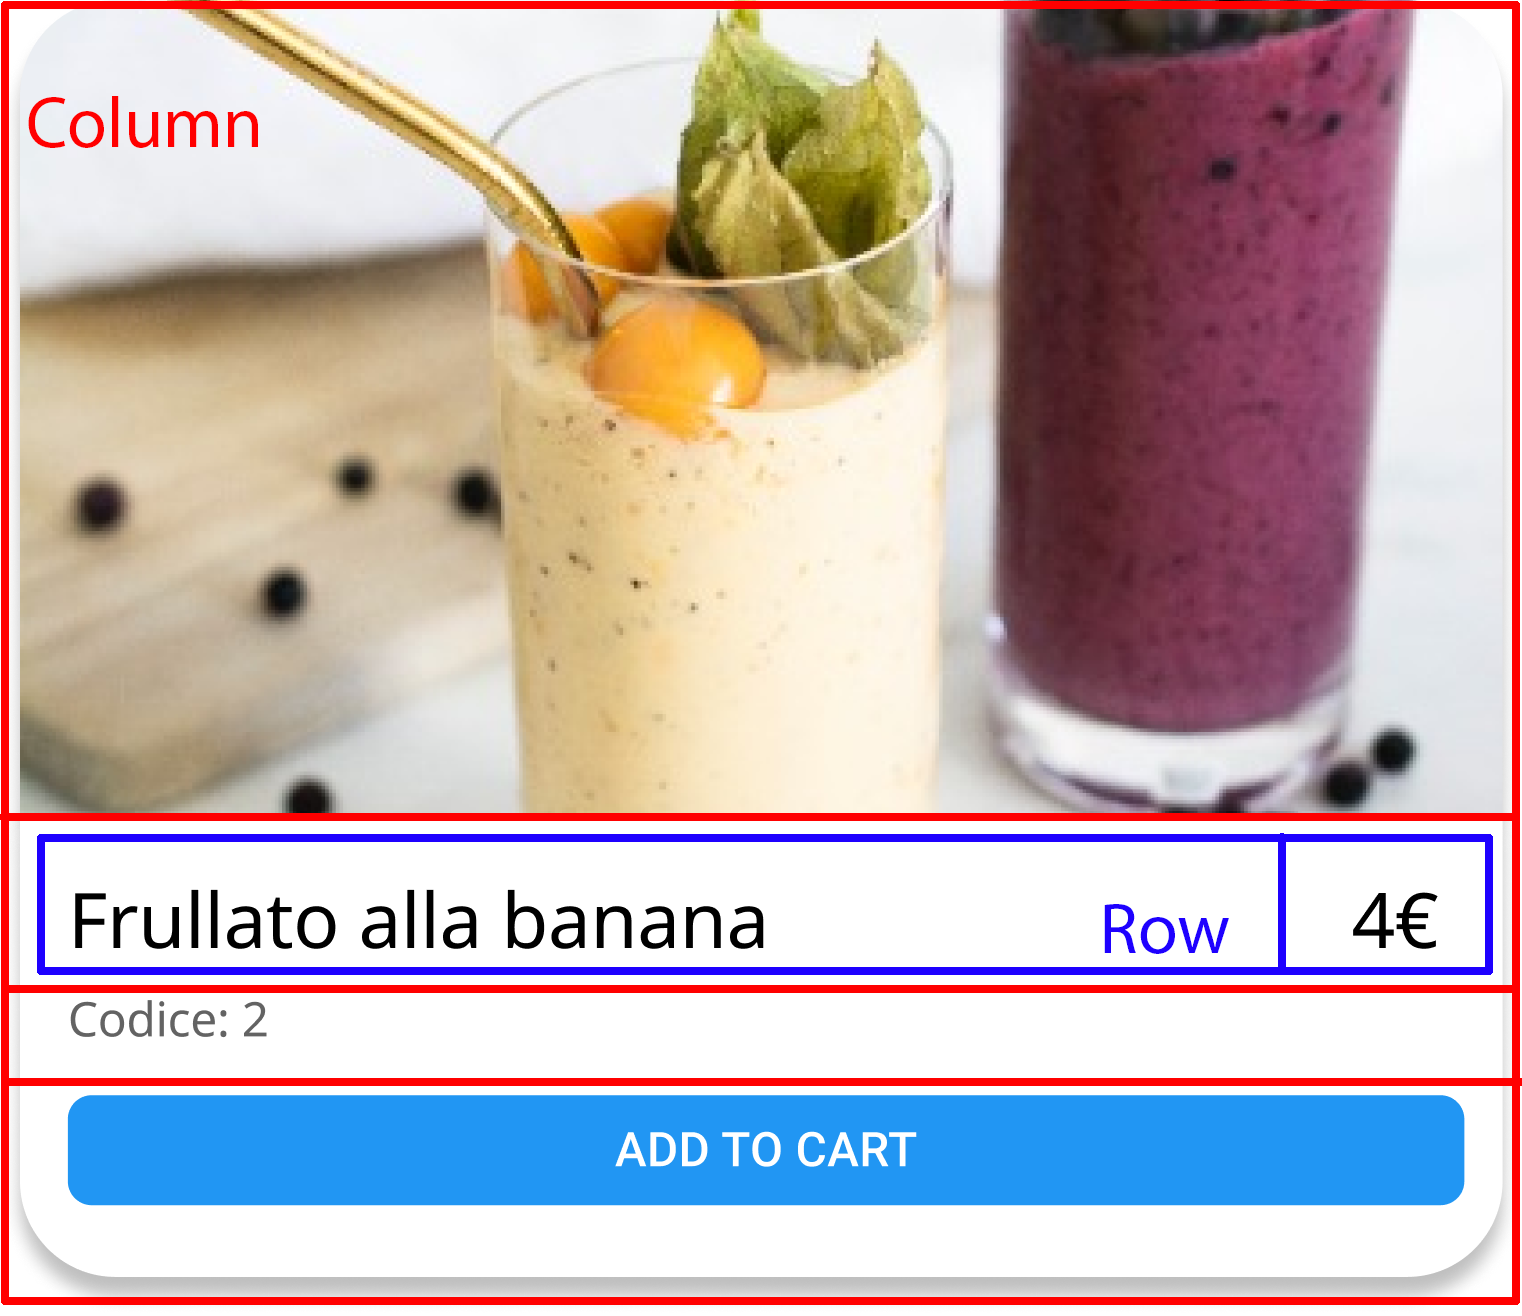
\includegraphics[width=\linewidth]{"Assets/card explained.png"}
	\end{minipage}
\end{figure}
Quindi dentro Column devono andare: la copertina se presente, Il Widget Row, che contiene a sua volta la descrizione e il prezzo unitario di vendita, l'id del prodotto e infine il pulsante. In pseudo-codice:
\begin{lstlisting}[language=Java][H]
Column(
	children: [
		if(url != null)
			Image.network(image_url),
		Row(
			children: [
				Text(desc),
				Text(price)
			]
		),
		Text(productId),
		RoundedLoadingButton(
			child: Text("ADD TO CART"),
			onPressed: () {
				// aggiungi al carrello
			}
		)
	]
)
\end{lstlisting}

\noindent
\subsubsection{Carrello}
Come è facile notare dalla \Cref{fig:figma_cart}, questa schermata presenta molte somiglianze con la pagina Home, in quanto ospita un elenco dinamico di Card. In aggiunta, vengono mostrati dettagli dell'importo totale e un pulsante per inoltrare l'ordine nella parte inferiore della schermata. Tuttavia, in questa situazione, le "Card" sono più complesse e richiedono un numero maggiore di elementi grafici anche se ci sono molte anolgie con le Card della schermata Home. La pagina è stata quindi divisa in questo modo
\begin{lstlisting}[language=Java, firstnumber=1][H]
Column (
	children : [
		ProductsList(),
		SubTotalAmount()
	]
)
\end{lstlisting}

\noindent
\paragraph{ProductsList}
Questa lista è molto simile a quella già descritta nella \Cref{par:listview}, ma il cambiamento principale sta proprio nelle Card: oltre ai soliti dati, quali descrizione del prodotto, codice, immagine facoltativa e prezzo unitario, è stata aggiunta la possibilità di modificare la quantità mediante 2 appositi pulsanti circolari insieme ad una label che mostra il prezzo totale dell'ordine (che corrisponde al prezzo unitario per la quantità). Inoltre i dati già descritti sono stati inseriti dentro un ListTile (vedi \Cref{cod:listile}). Per agevolare la comprensione al lettore, allego un'immagine esplicativa che illustra la progettazione dell'interfaccia utente in modo più semplice e chiara:
\begin{flushleft}
	\begin{minipage}[t]{1\linewidth}
		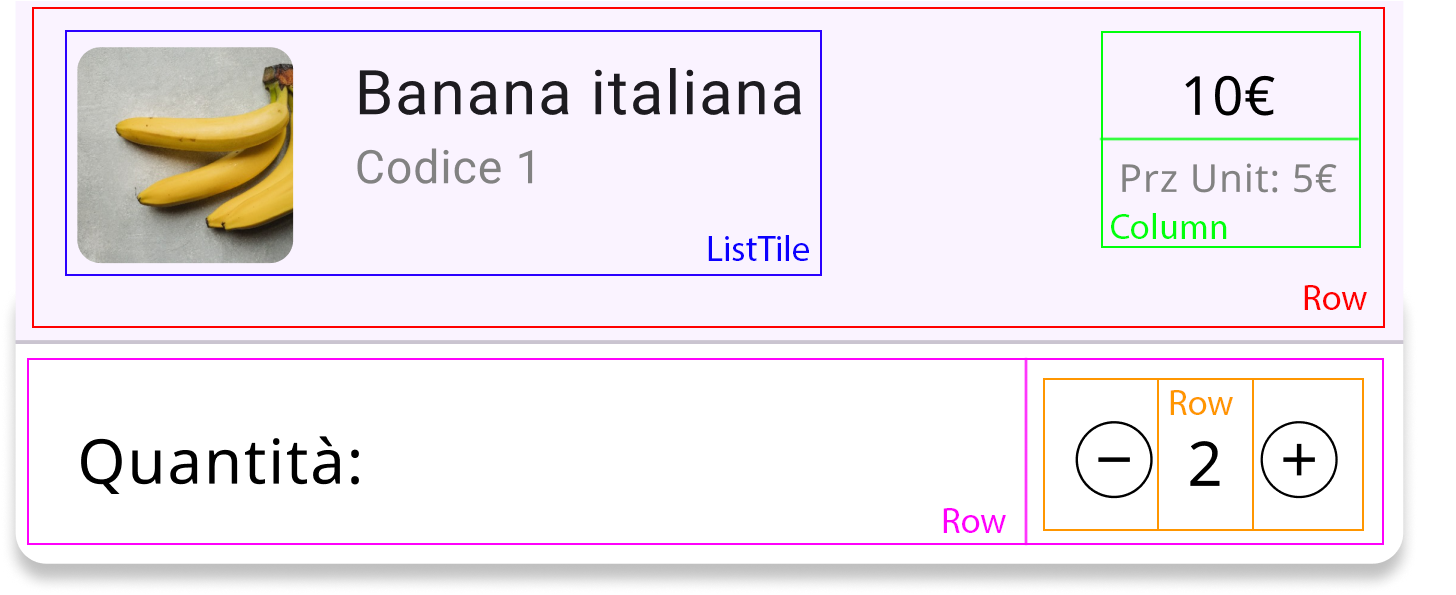
\includegraphics[width=\linewidth]{"Assets/complex list item.png"}
		\label{fig:complexCard}
	\end{minipage}
\end{flushleft}

\noindent
In codice:
\begin{lstlisting}[language=Java, firstnumber=1][H]
Column(
	children: [
		Row(
			children: [
				Expanded(
					ListTile(...),
				),
				Column(
					children: [
						Text(price),
						Text(priceUnit),
					]
				)
			
			]
		),
		Row(
			children: [
				Expanded(
					Text("Quantity"),
				),
				Row(
					children: [
						IconButton(...), // aggiungi quantita'
						Text(quantity),
						IconButton(...), // rimuovi quantita'
					]
				)
			]
		)
	]
)
\end{lstlisting}

\noindent
Piccola nota di rilievo va al ListTile (quadrato blu della figura sopra) che è stato sviluppato come segue:
\begin{lstlisting}[language=Java, firstnumber=122][H]
ListTile(
	leading: imgUrl != null ? Image.network(umgUrl) : null,
	title: const Text(desc),
	subtitle: const text(productId)
)
\end{lstlisting}

\noindent
Mentre la label "Quantità" della \Cref{fig:complexCard} è stata inserita dentro un Widget Expanded in modo che la seconda riga, quella che contiene i pulsanti per modificare la quantità, si spostasse tutta a destra.
Queste Card hanno infine la peculiarità di essere dismissible: l'utente può trascinare verso sinistra o destra una di esse per rimuovere l'ordine dal carrello. Per far ciò basta inserire la Card dentro un Widget di tipo Dismissible, in questo modo:
\begin{lstlisting}[language=Java, firstnumber=1][H]
Dismissable(
	child: Card(...)
)
\end{lstlisting}

\noindent

\paragraph{SubTotalAmount}
La parte dedicata al display del prezzo totale occupa una porzione fissa all'interno della schermata: di fatto, allo scorrere della lista, questa non si muove con essa. Lo sviluppo è molto semplice, di fatto è una Row (che contiene le due label "Sub-Total" e il prezzo, vedi \Cref{fig:figma_cart}) dentro un Widget Column. In codice:
\begin{lstlisting}[language=Java, firstnumber=1][H]
Column(
	children: [
		Row(
			children: [
				Expanded(
					child: Text("Sub Total"),
				),
				Expanded(
					child: Text(totalPrice)
				)
			]
		)
	],
	ElevatedButton(
		child: Text("Submit Order")
	)
)
\end{lstlisting}

\noindent
\subsubsection{Profilo}
Come illustrato in \Cref{fig:figma_profile}, la schermata del profilo presenta un'immagine con il relativo username posizionato appena sotto di essa. Le informazioni dell'utente sono organizzate in una breve lista, e vi è un pulsante "logout" di colore rosso. Ho scelto di adottare questa disposizione poiché le informazioni disponibili nel Database sono limitate, e ho cercato quindi di ottimizzare l'utilizzo dello spazio a mia disposizione. In realtà, con ulteriori informazioni, potrebbe essere opportuno considerare l'opzione di unire i campi "nome" e "cognome" in un'unica etichetta.\\
Nota: è importante precisare che l'indirizzo email e la foto del profilo vengono attualmente inseriti a scopo illustrativo e non sono effettivamente ricevuti dal Server. In codice:
\begin{lstlisting}[language=Java, firstnumber=1][H]
Expanded(
	child: Column(
		children: [
			Expanded(
				flex: 1,
				ClipOval(
					child: FadeInImage(
						image: const NetworkImage(url),
						imageErrorBuilder: (context, error, stackTrace) {
							return const CircleAvatar(
								backgroundImage: AssetImage("profile.png")
							);
						}
					)
				),
				Text(username),
			),
			Expanded(
				flex: 2,
				child: Column(
					children: [
						Text(name),
						Text(surname)
					]
				)
			),
			Expanded(
				child: ElevatedButton(child: Text("LOGOUT"))
			)
		]
	)

)	
\end{lstlisting}

\noindent
Un dettaglio da sottolineare riguarda l'utilizzo dei valori "flex: 1" e "flex: 2". Questi parametri definiscono la quantità di spazio che i Widget sono autorizzati a occupare all'interno del layout. Di norma, tutti i Widget hanno un valore predefinito di "flex: 1", il che significa che si distribuiranno equamente nello spazio disponibile. La lista, tuttavia, che visualizza le informazioni dell'utente, richiede più spazio rispetto all'immagine e al testo sottostante posizionati nella parte superiore della pagina, per questo le è assegnato un valore "flex: 2". Per approfondire meglio invece l'utilizzo di "FadeInImage", rimando il lettore al \Cref{subsub:fadeinimage}.

\subsection{Comunicazione tra Widget} \label{lab_widget_communication}
Per la comunicazione tra i vari Widget viene utilizzata la classe "SharedProvider" (vedi \Cref{subsub:provider}). Essa assume un ruolo di rilievo nell'orchestrare la comunicazione efficace tra i Widget Flutter. In particolare, la sua funzione centrale è quella di facilitare la condivisione di dati e lo scambio di informazioni tra diverse parti dell'applicazione, contribuendo a mantenere uno stato coerente e sincronizzato tra i vari componenti.\\
In particolare questa classe memorizza:
\begin{itemize}
	\item Token di accesso e aggiornamento,
	\item Carrello utente,
	\item Articoli cercati dall'utente che sono restituiti dal Server,
	\item Testata corrente,
	\item Importo complessivo dei prodotti presenti nel carrello.
\end{itemize}

\noindent
\paragraph{Creazione di SharedProvider}
Questa classe estende ChangeNotifier della libreria Provider e la sua creazione avviene all'avvio dell'applicazione subito dopo il main:
\begin{lstlisting}[language=Java, firstnumber=1][H]
	void main() {
		runApp(const CompanionApp());
	}
	
	class CompanionApp extends StatefulWidget {
		const CompanionApp({super.key});
		
		@override
		State<CompanionApp> createState() => CompanionAppState();
	}
	
	class CompanionAppState extends State<CompanionApp> {

		@override
		Widget build(BuildContext context) {
			return MultiProvider(
			providers: [
				ChangeNotifierProvider(
					create: (.) => SharedProvider()
				),
			],
			...
		}
\end{lstlisting}

\noindent
A questo punto il Provider è disponibile in qualsiasi punto dell'applicazione, richiedibile mediante:
\begin{lstlisting}[language=Java, style=longBlock, firstnumber=1][H]
	SharedProvider p = Provider.of<SharedProvider>(context, listen: false);
	
	// in caso non sia disponibile il contesto context:
	WidgetsBinding.instance.addPostFrameCallback((timeStamp) {
		SharedProvider provider = Provider.of<SharedProvider>(context, listen: false);
	});
\end{lstlisting}

\noindent
Per semplicità e compattezza, è stato implementato un metodo statico (detto anche "stub") all'interno della classe SharedProvider. Questo metodo è stato progettato appositamente per agevolare l'accesso al Provider in maniera diretta e immediata, richiedendo solamente il parametro di tipo BuildContext\footnote{Classe astratta di Flutter che rappresenta il cuore di un Widget. Un BuildContext in Flutter è un oggetto che fornisce informazioni sulla posizione di un Widget all'interno del "Widget Tree". È essenziale per accedere a risorse e dati specifici del Widget, infatti ogni Widget è associato ad un BuildContext.}:
\begin{lstlisting}[language=Java][H]
factory SharedProvider.getInstance(BuildContext context) {
	return Provider.of<SharedProvider>(context, listen: false);
}
\end{lstlisting}

\noindent
\paragraph{Caricamento dei dati}
All'avvio dell'applicazione vengono lette e caricate le informazioni utente dal disco fisico dentro la classe SharedProvider poichè questa operazione assicura che, durante l'intero ciclo di vita dell'applicazione, le informazioni necessarie per il suo corretto funzionamento siano prontamente accessibili. In pseudo-codice:
\begin{lstlisting}[language=Java, firstnumber=1][H]
Map<String, Object> initData = loadFromDisk();

String accessToken = initData['access_token'];
String refreshToken = initData['refresh_token'];
int currentTestataId = initData['currentTestataId'];
List<Order> cart = initData['cart'];

SharedProvider provider = SharedProvider.getInstance(context);
provider.accessToken = accessToken;
provider.refreshToken = refreshToken;
provider.currentTestataId = currentTestataId;
provider.cartProducts = cart;
\end{lstlisting}

\noindent
Un esempio concreto è la situazione in cui vi sia la necessità di recuperare il token di accesso. In tal caso, basta seguire la sequenza di istruzioni di seguito riportata:
\begin{lstlisting}[language=Java, firstnumber=1][H]
SharedProvider provider = SharedProvider.getInstance(context);

const accessToken = provider.accessToken;
\end{lstlisting}

\noindent
\paragraph{Aggiornamento UI}
Per fare in modo che gli elementi dell'interfaccia utente si aggiornino quando si verificano dei cambiamenti, è essenziale inserirli nell'oggetto di tipo "Selector" (vedi \Cref{subsub:provider}). Un esempio può essere l'aggiornamento del prezzo totale della testata ogni qual volta l'utente inserisce un prodotto nuovo al carrello o modifica la quantità di un ordine:
\begin{lstlisting}[language=Java, firstnumber=1][H]
	child: Selector<SharedProvider, double>(
		selector: (context, provider) => provider.cartTotalPrice,
		builder: (context, cartTotalPrice, child) {
			return Text(cartTotalPrice);
		}
	)
\end{lstlisting}

\noindent
In questo caso, il parametro "selector" prende in input il prezzo totale del carrello cosicché, quando questo cambia, la funzione passata al parametro "builder" venga usata per aggiornare l'interfaccia utente con il nuovo dato.
Per notificare il cambiamento, basta invocare il metodo:
\begin{lstlisting}[language=Java, firstnumber=1][H]
	notifyListeners();
\end{lstlisting}

\noindent
ereditato dalla classe ChangeNotifier. Sempre in riferimento all'esempio mostrato sopra, quindi, per aggiornare il prezzo totale della testata basta inserire dentro la classe SharedProvider:
\begin{lstlisting}[language=Java, firstnumber=1][H]
	void setTotalPrice(double price) {
		cartTotalPrice = price;
		notifyListeners();
	}
\end{lstlisting}

\noindent
A questo punto, una volta invocato il metodo sopra, il Selector noterà la differenza con il valore precedente e invocherà la funzione passata al parametro "builder" per aggiornare l'interfaccia.\\
Questo approccio assicura un notevole livello di efficienza e contribuisce a una drastica riduzione del consumo energetico, un aspetto di cruciale importanza nel contesto dello sviluppo di applicazioni mobili. Inoltre viene ridotto significativamente il carico computazionale richiesto per aggiornare la UI, poiché vengono evitate le ricostruzioni inutili e, di conseguenza, si riscontra una diminuzione sostanziale nell'utilizzo di risorse, tra cui CPU e memoria (ciò è particolarmente rilevante nei dispositivi mobili, dove le risorse sono spesso limitate). Infine, l'adozione di tale approccio consente di garantire una risposta più rapida agli aggiornamenti dei dati, poiché solo le porzioni rilevanti dell'interfaccia vengono adeguatamente aggiornate.\\ Questo si traduce in un'esperienza utente più fluida e reattiva, contribuendo a migliorare la percezione complessiva dell'applicazione da parte degli utenti.

\subsection{Asincronia delle richieste}
L'applicazione fa un ampio utilizzo delle chiamate asincrone, poiché spesso è necessario comunicare con il Server e, attendere sempre la risposta, causerebbe un blocco totale dell'applicazione, il che è altamente irrealistico. Tuttavia, sorge il problema che in molte occasioni è necessario visualizzare un'interfaccia ancor prima di aver ottenuto i dati necessari per popolarla.
Per superare questa difficoltà, Flutter mette a disposizione il Widget FutureBuilder, che è stato impiegato per presentare all'utente un'interfaccia predefinita mentre si attende il completamento del caricamento dei dati dal Server. Un esempio concreto si manifesta nella pagina del carrello: fintanto che l'elenco dei contenuti corretto non è disponibile, viene mostrato l'ultimo elenco ricevuto salvato localmente. Il seguente codice ne rappresenta un esempio:
\begin{lstlisting}[language=Java, style=longBlock, firstnumber=1][H]
body: FutureBuilder<List<Order>>(
		future: getCart(),
		initialData: SharedProvider.getInstance(context).cartProducts,
		builder: (context, snapshot) {
			if (!snapshot.hasData) {
				return const LoadingPage();
			}
			
			// lista pronta
			List<Order> list = snapshot.data;
		}
	)
	
Future<List<Order>> getCart() async {
	// richiesta HTTP per prendere il carrello in modo asincrono
}
\end{lstlisting}

\noindent
Nell'esempio sopra, si evidenzia la potenza del FutureBuilder: mentre il carrello viene recuperato dal Server attraverso la funzione "getCart()", il Widget utilizza dati iniziali per mostrare istantaneamente "qualcosa" all'utente. Questo "qualcosa" corrisponde alla lista più recente di ordini ricevuta dal Server e memorizzata localmente (tutto ciò avviene senza interferire con il processo di scaricamento in background). In questo contesto, il valore "snapshot.data" rappresenta l'initialData, ossia la lista locale e, una volta che il Client riceve effettivamente il carrello, il FutureBuilder invoca il metodo definito nel parametro "builder" con lo snapshot che conterrà i dati scaricati attraverso il metodo "getCart()", anziché i dati locali precedentemente visualizzati. L'if è stato messo a scopo difensivo, in quanto è possibile che non esista nessuna lista localmente e che il tempo di scaricamento sia prolungato.\\
Per concludere, un ulteriore e importante strato di asincronia è stato adottato nell'esecuzione delle richieste HTTP, con incluse le relative gestioni dei timeout. Queste operazioni avvengono in background, una scelta guidata dalla necessità di ottimizzare le performance complessive dell'applicazione. L'interfaccia tra l'app e il protocollo HTTP è stata gestita attraverso la classe astratta "NetworkUtility": questo oggetto non solo esegue i controlli per la validità dei token (in più, nel caso in cui il token di accesso sia scaduto, la classe ne richiederà immediatamente, al Server, uno nuovo) prima di inoltrare la richiesta, ma si occupa anche di presentare eventuali messaggi di errore all'utente mediante l'uso di material dialog.

\subsection{Persistenza su disco}
Per quanto riguarda la memorizzazione delle informazioni dell'utente e dell'ultimo carrello ricevuto dal Server, è stato adottato il framework SQLite. Tali dati vengono archiviati su disco all'interno di apposite tabelle, create appositamente per questa finalità. La struttura del Database è generata secondo la seguente procedura:
\begin{lstlisting}[language=SQL, style=longBlock, firstnumber=1][H]
    openDatabase(
        join(await getDatabasesPath(), 'companion.db'),
        version: 1, onCreate: (db, version) async {
      await db.execute(
        'CREATE TABLE User(id INTEGER PRIMARY KEY, name TEXT, surname TEXT, creationDate TEXT, username TEXT)');
      return db.execute(
        'CREATE TABLE Products(id INTEGER PRIMARY KEY, desc TEXT, price REAL, quantity INTEGER, imageUrl TEXT)',
      );
    });
\end{lstlisting}

\noindent
Ora è intuitivo concepire che le informazioni dell'utente siano conservate nella prima tabella denominata "User", mentre i prodotti nel carrello trovano collocazione nella seconda tabella chiamata "Products". Dato che è necessario archiviare oggetti all'interno del Database, ho seguito il consiglio proveniente dalla documentazione di Flutter, pertanto, ho implementato due metodi che permettono la conversione dell'oggetto in una struttura di tipo mappa (Map) e la successiva ricostruzione dell'oggetto a partire da questa. Il procedimento si articola nel seguente modo:
\newpage
\begin{lstlisting}[language=Java, firstnumber=1][H]
class User {
  final String name;
  final String surname;
  final String creationDate;
  final String username;

  User(this.name, this.surname, this.creationDate, this.username);

  factory User.fromMap(Map<String, dynamic> json) {
    return User(
      json['name'],
      json['surname'],
      json['creationDate'],
      json['username'],
    );
  }

  Map<String, Object?> toMap() {
    return {
      "name" : name,
      "surname" : surname,
      "creationDate" : creationDate,
      "username" : username,
    };
  }
}
\end{lstlisting}

\noindent
Per inserire i dati nel Database è stato usato questo metodo:
\begin{lstlisting}[language=Java, style=longBlock, firstnumber=1][H]
	db.insert(userTable, user.toMap(), conflictAlgorithm: ConflictAlgorithm.replace);
\end{lstlisting}

\noindent
E per riottenerli, basta usare il seguente approccio:
\begin{lstlisting}[language=java, style=longBlock, firstnumber=1][H]
    final List<Map<String, dynamic>> maps = await db.query(userTable);
    User u = User.fromMap(maps[0]);
\end{lstlisting}

\noindent
Ovvero leggere i dati come una Map e passarla al costruttore definito inizialmente.\\
Infine, la lista del carrello è memorizzata mediante l'utilizzo di una transazione, il che permette di tornare alla lista precedente in caso di eventuali errori. In codice:
\begin{lstlisting}[language=Java, firstnumber=1][H]
Batch batch = db.batch();

for (Order p in cartProducts) {
	// in caso di errore, il batch annulla la transazione
	try{
		batch.insert(productsTable, p.toMap(), conflictAlgorithm: ConflictAlgorithm.replace);
	}catch(error) {
		return;
	}
}

await batch.commit(noResult: true);	
\end{lstlisting}

\noindent

\subsection{Deeplink}\label{sub:deeplink}
Veniamo ora ad una delle parti più fondamentali dell'applicazione, i Deeplink. Come descritto all'inizio del \Cref{chapter_sviluppo_app}, ci sono 3 tipi di Deeplink che l'applicativo deve gestire:
\begin{itemize}
\item \textbf{info01://codice01.companion.it/token}\\ esegue il login automatico
\item \textbf{info01://codice01.companion.it/token/code=?}\\ esegue il login automatico, aggiunge al carrello il prodotto con codice specificato e imposta la quantità ad 1, accedendo direttamente alla pagina del carrello
\item \textbf{info01://codice01.companion.it/token/code=?/quantity=?}\\ uguale al punto precedente, con l'unica differenza che la quantità è specificata
\end{itemize}

\noindent
Per lo sviluppo è stata usata la libreria "go\_router" (vedi \Cref{subsub:go_router}), che si rivela eccellente poiché gestisce la ricezione dei Deeplink in maniera naturale e veloce, offrendo un'esperienza di integrazione molto fluida e rendendo semplice il parsing dell'URI.
\paragraph{Definizione dello schema} Affinché si riesca a catturare quel particolare tipo di URI ("info01://codice01.companion.it"), è necessario settare il tipo di schema e host che si vuole usare. Per far ciò bisogna modificare l "AndroidManifest.xml" (per Android) e l "info.plist" (per iOS) secondo le direttive dettate dal sito di Flutter.\\
In particolare è necessario aggiungere queste righe all "AndroidManifest.xml":
\begin{lstlisting}[language=XML, style=longBlock, firstnumber=1][H]
	<meta-data android:name="flutter_deeplinking_enabled" android:value="true"/>
	<intent-filter android:autoVerify="true">
	<action android:name="android.intent.action.VIEW" />
	<category android:name="android.intent.category.DEFAULT" />
	<category android:name="android.intent.category.BROWSABLE" />
	<data android:scheme="http"/>
	<data android:scheme="info01"/>
	<data android:host="codice01.companion.it"/>
\end{lstlisting}

\newpage
\noindent
E queste per l "info.plist":
\begin{lstlisting}[language=Java, firstnumber=1][H]
<key>FlutterDeepLinkingEnabled</key>
<true/>
<key>CFBundleURLTypes</key>
<array>
    <dict>
    <key>CFBundleTypeRole</key>
    <string>Editor</string>
    <key>CFBundleURLName</key>
    <string>codice01.companion.it</string>
    <key>CFBundleURLSchemes</key>
    <array>
    <string>info01</string>
    </array>
    </dict>
</array>
\end{lstlisting}

\noindent
\paragraph{Definizione delle rotte}
Per garantire che l'applicazione risponda correttamente quando l'utente preme su un Deeplink, è essenziale istituire delle "rotte". Queste rotte rappresentano dei veri e propri punti di accesso che ricevono l'URI, lo analizzano tramite parsing e restituiscono i risultati appropriati. Questo compito può essere agevolato utilizzando la libreria "go\_router", menzionata in precedenza. Tale libreria include dei Widget appositamente progettati per definire queste rotte e specificare quali parametri devono essere presenti nell'URI. Nello specifico, la definizione di una rotta segue il seguente schema:
\begin{lstlisting}[language=Java, firstnumber=1][H]
GoRoute(
	path: "/:token/code=:cd",
	name: "token_product_add",
	builder: (context, state) {
		String token = state.pathParameters['token'];
		int code = int.parse(state.pathParameters['cd']);
	},
),
\end{lstlisting}

\noindent
In cui ":token" e ":cd" rappresentano due parametri della mappa "state.pathParameters" e questi vengono sottoposti a parsing nel momento in cui il sistema identifica che un deeplink corrisponde a una delle rotte definite. In conclusione, quindi, i 3 punti richiesti sono così definiti:
\newpage
\begin{lstlisting}[language=Java][H]
[
	GoRoute(
		path: "/:token",
		name: "token_home",
		builder: (context, state) {
			// login automatico
		},
	),
	GoRoute(
		path: "/:token/code=:cd",
		name: "token_product_add",
		builder: (context, state) {
			// login automatico e aggiunta prodotto nel carrello
		},
	),
	GoRoute(
		path: "/:token/code=:cd/quantity=:qt",
		name: "token_product_add_quantity",
		builder: (context, state) {
			// login automatico e aggiunta prodotto nel carrello
			// con quantita'
		},
	),
]
\end{lstlisting}

\noindent
Questo array di "GoRoute", infine, deve essere passato come parametro al Widget root del MaterialApp\footnote{Il punto di partenza di ogni applicazione Flutter. MaterialApp è un Widget che permette di definire il tema, la navigazione tra le schermate, la lingua ecc. Solitamente le impostazioni base vengono definite tramite questo Widget.} denominato "MaterialApp.router" in questo modo:
\begin{lstlisting}[language=Java, firstnumber=1][H]
MaterialApp.router(
	routerConfig: GoRouter(
		routes: [
			GoRoute(...),
			GoRoute(...),
			GoRoute(...),
		]
	)
)
\end{lstlisting}

\noindent
Adesso quando l'utente cliccherà, per esempio, su questo link:
\begin{lstlisting}[language=Java][H]
info01://codice01.companion.it/123456789/code=10/quantity=12
\end{lstlisting}

\noindent
La pagina del carrello si aprirà automaticamente, presentando il prodotto con codice 10 già inserito e con una quantità preimpostata di 12 (supponendo che il token sia valido ovviamente).

\subsection{Animazioni}
L'applicazione fa ampio uso delle animazioni in quanto contribuiscono alla resa visiva generale e rendono più piacevole l'esperienza d uso. Al fine di integrare in modo efficace queste animazioni all'interno dell'applicazione, è stata adottata la libreria Lottie, che permette di visualizzare brevi sequenze animate, attraverso file JSON, scaricabili dal suo sito ufficiale e che aiutano gli utenti a comprendere meglio cosa sta avvenendo.
In particolare, le animazioni di Lottie sono state impiegate in modo predominante nei Dialog, sfruttando la libreria "Material Dialog" e "Lottie". Questo approccio è stato adottato sia quando un utente completa con successo un ordine, sia in caso si verifichino eventuali errori, come ad esempio la mancata connessione al Server, il reindirizzamento a una pagina inesistente tramite deeplink, il termine della sessione o in caso di errore generico. I file JSON, contenenti le descrizioni delle animazioni, vengono tutti archiviati nella cartella "lib/lottie" e successivamente passati come argomento al parametro "lottieBuilder", come illustrato qui sotto:
\begin{lstlisting}[language=Java, firstnumber=1][H]
Dialogs.materialDialog(
	lottieBuilder: Lottie.asset("lottie_animation.json")
)	
\end{lstlisting}

\noindent
\chapter{Conclusioni}
In questo documento si è delineato l'intero processo di sviluppo di un'applicazione mobile, sia lato back-end che front-end, che fa uso sia di approcci più tradizionali sia sfruttando l'utilizzo dei deeplink. L'obiettivo principale è stato, quindi, la creazione di un'applicazione, denominata Companion, che consentisse agli utenti di effettuare acquisti in modo agevole, sfruttando questo approccio ibrido: da un lato, sono state implementate funzionalità più tradizionali, come la ricerca e l'acquisto mediante l'uso di una barra di ricerca e di un carrello, mentre dall'altro si è sfruttato l'uso dei deeplink come dettagliato nella \Cref{sub:deeplink}, al fine di facilitare l'esperienza utente, in quanto consentono agli utenti di acquistare i prodotti dal catalogo cliccando su un semplice URL. Si sottolinea che ogni utente ha avuto accesso a un listino prezzi dedicato, come descritto esaustivamente nella \Cref{section2}.
Per quanto riguarda il lato back-end, il Server è stato implementato con una gestione multithreading in grado di gestire contemporaneamente multiple richieste. Questo è stato realizzato utilizzando la libreria Javalin, come descritto nella \Cref{subsub:javalin} e l'adozione dei JSON Web Token, che hanno reso il sistema altamente scalabile in quanto le informazioni sugli utenti non sono memorizzate direttamente sul disco, ma dentro questi token come ampiamente descritto nella sezione \Cref{section_token}.\\
Companion è quindi un'applicazione su misura, sviluppata per soddisfare le specifiche esigenze di un cliente in particolare.
Un obiettivo significativo raggiunto riguarda l'adozione di Javalin come framework lato Server: l'ottimizzazione delle risorse di memoria ha permesso di ottenere un'applicazione reattiva, leggera e, inoltre, la persistenza su disco si è dimostrata preziosa per garantire la continuità dell'applicazione anche in caso di chiusura inattesa del Server (vedi \Cref{subsub:key_creation_and_disk_persistency}).
Nel complesso, si è cercato di adottare un approccio efficiente nello sviluppo, scegliendo algoritmi con complessità ottimale e evitando scenari di tempo computazionalmente elevato ($O(n^2)$). Inoltre, lato Client, è stata ottimizzata l'efficienza minimizzando la ricostruzione dei Widget quando non strettamente necessario.

\section{Funzionalità future e possibili miglioramenti}
Essendo Companion un'applicazione orientata alla facilità di acquisto dei prodotti, alcune funzionalità aggiuntive possono essere: una cronologia degli acquisti, in grado di mostrare agli utenti cosa hanno comprato in passato (e quindi di poterle ricomprare), la capacità di scannerizzare con la fotocamera un codice a barre personalizzato creato dall'azienda, al fine di aggiungere automaticamente un prodotto al carrello e, infine, la possibilità di inserire manualmente la quantità di un prodotto senza l'ausilio dei pulsanti nella pagina del carrello.\\
Come accennato in precedenza, la classe 'Provider' è stata utilizzata in modo estensivo per facilitare la comunicazione tra i Widget; tuttavia, con l'esperienza accumulata, ritengo che in futuro sia necessario optare per alternative diverse a questo framework, poiché è stato riscontrato che il suo utilizzo può risultare tedioso in diverse circostanze, sopratutto riguardo alla necessità di avere un "context", ovvero un oggetto chiave di Flutter per accedere all'oggetto globale e questa dipendenza può portare a molteplici verifiche quando si gestiscono chiamate asincrone, in quanto questo oggetto potrebbe desistere in qualunque momento.
Lato Server, l'esperienza con Javalin è stata stimolante e di semplice comprensione, tuttavia, in scenari reali, probabilmente sarebbe preferibile utilizzare framework più robusti ed efficienti, dato che esistono alcune funzionalità essenziali mancanti di completezza (per esempio, il supporto a HTTPS non è pienamente supportato)

\section{Considerazioni sul tirocinio}
Nello svolgimento del tirocinio, sono stati appresi diversi strumenti che durante il percorso universitario non è stato possibile conoscere. In particolare, l'uso dei token JWT e il linguaggio Flutter sono le due principali caratteristiche che sono state apprezzate di più, in quanto Flutter permette di scrivere un applicazione una volta e averla su più piattaforme, mentre JWT ha il grande vantaggio di facilitare la reperibilità dei dati importanti.\\ Il tirocinio in generale ha permesso quindi di conoscere tecnologie nuove e di poter sviluppare un applicativo effettivamente usabile da un azienda per poter vendere ai suoi clienti i propri prodotti.

\appendix
% \chapter{Questa è un'appendice}

\lipsum[5]

\section*{Questa è un'altra sezione, ma non viene inserita nell'indice}

\lipsum[6]

\bibliographystyle{plain}
\bibliography{Capitoli/Utility/Bibliografia}

\end{document}
% -----------------------------------------------------------------
